\documentclass[12pt,a4paper]{report}

\usepackage[utf8]{inputenc} % pentru suport diacritice
\usepackage[english]{babel} % setări pentru limba engleza 
\renewcommand\familydefault{\sfdefault} % sans serif

\usepackage[margin=2.54cm]{geometry}	% dimensiuni pagină și margini
\usepackage{graphicx} % support the \includegraphics command and options

% formatting sections and subsections
\usepackage{textcase}
\usepackage{hyphenat}
\usepackage[titletoc, title]{appendix}
\usepackage{titlesec}
\titleformat{\chapter}{\large\bfseries\MakeUppercase}{\thechapter}{2ex}{}[\vspace*{-1.5cm}]
\titleformat*{\section}{\large\bfseries}
\titleformat*{\subsection}{\large\bfseries}
\titleformat*{\subsubsection}{\large\bfseries}

\usepackage{chngcntr}
\counterwithout{figure}{chapter} % no chapter number in figure labels
\counterwithout{table}{chapter} % no chapter number in table labels
\counterwithout{equation}{chapter} % no chapter number in equation labels

\usepackage{booktabs} % for much better looking tables
\usepackage{url} % Useful for inserting web links nicely
\usepackage[bookmarks,
			unicode,
			hidelinks,
			colorlinks = true,
			anchorcolor = blue,
			linkcolor = black,
			urlcolor = blue]{hyperref}

\usepackage{array} % for better arrays (eg matrices) in maths
\usepackage{paralist} % very flexible & customisable lists (eg. enumerate/itemize, etc.)
\usepackage{verbatim} % adds environment for commenting out blocks of text & for better verbatim
\usepackage{subfig} % make it possible to include more than one captioned figure/table in a single float
\usepackage{enumitem}
\setlist{noitemsep}

%%% HEADERS & FOOTERS
\usepackage{fancyhdr}
\pagestyle{empty}
\renewcommand{\headrulewidth}{0pt}
\renewcommand{\footrulewidth}{0pt}
\lhead{}\chead{}\rhead{}
\lfoot{}\cfoot{\thepage}\rfoot{}



\newcommand{\HeaderLineSpace}{-0.25cm}
\newcommand{\UniTextRO}{UNIVERSITATEA POLITEHNICA DIN BUCUREȘTI \\[\HeaderLineSpace] 
FACULTATEA DE AUTOMATICĂ ȘI CALCULATOARE \\[\HeaderLineSpace]
DEPARTAMENTUL DE CALCULATOARE\\}
\newcommand{\DiplomaRO}{PROIECT DE DIPLOMĂ}
\newcommand{\AdvisorRO}{Coordonator științific:}
\newcommand{\BucRO}{BUCUREȘTI}

\newcommand{\UniTextEN}{UNIVERSITY POLITEHNICA OF BUCHAREST \\[\HeaderLineSpace]
FACULTY OF AUTOMATIC CONTROL AND COMPUTERS \\[\HeaderLineSpace]
COMPUTER SCIENCE AND ENGINEERING DEPARTMENT\\}
\newcommand{\DiplomaEN}{DIPLOMA PROJECT}
\newcommand{\AdvisorEN}{Thesis advisor:}
\newcommand{\BucEN}{BUCHAREST}

\newcommand{\frontPage}[6]{
\begin{titlepage}
\begin{center}
{\Large #1}  % header (university, faculty, department)
\vspace{50pt}
\begin{tabular}{p{6cm}p{4cm}}

\includegraphics[scale=0.8]{pics/upb-logo.jpg} &
	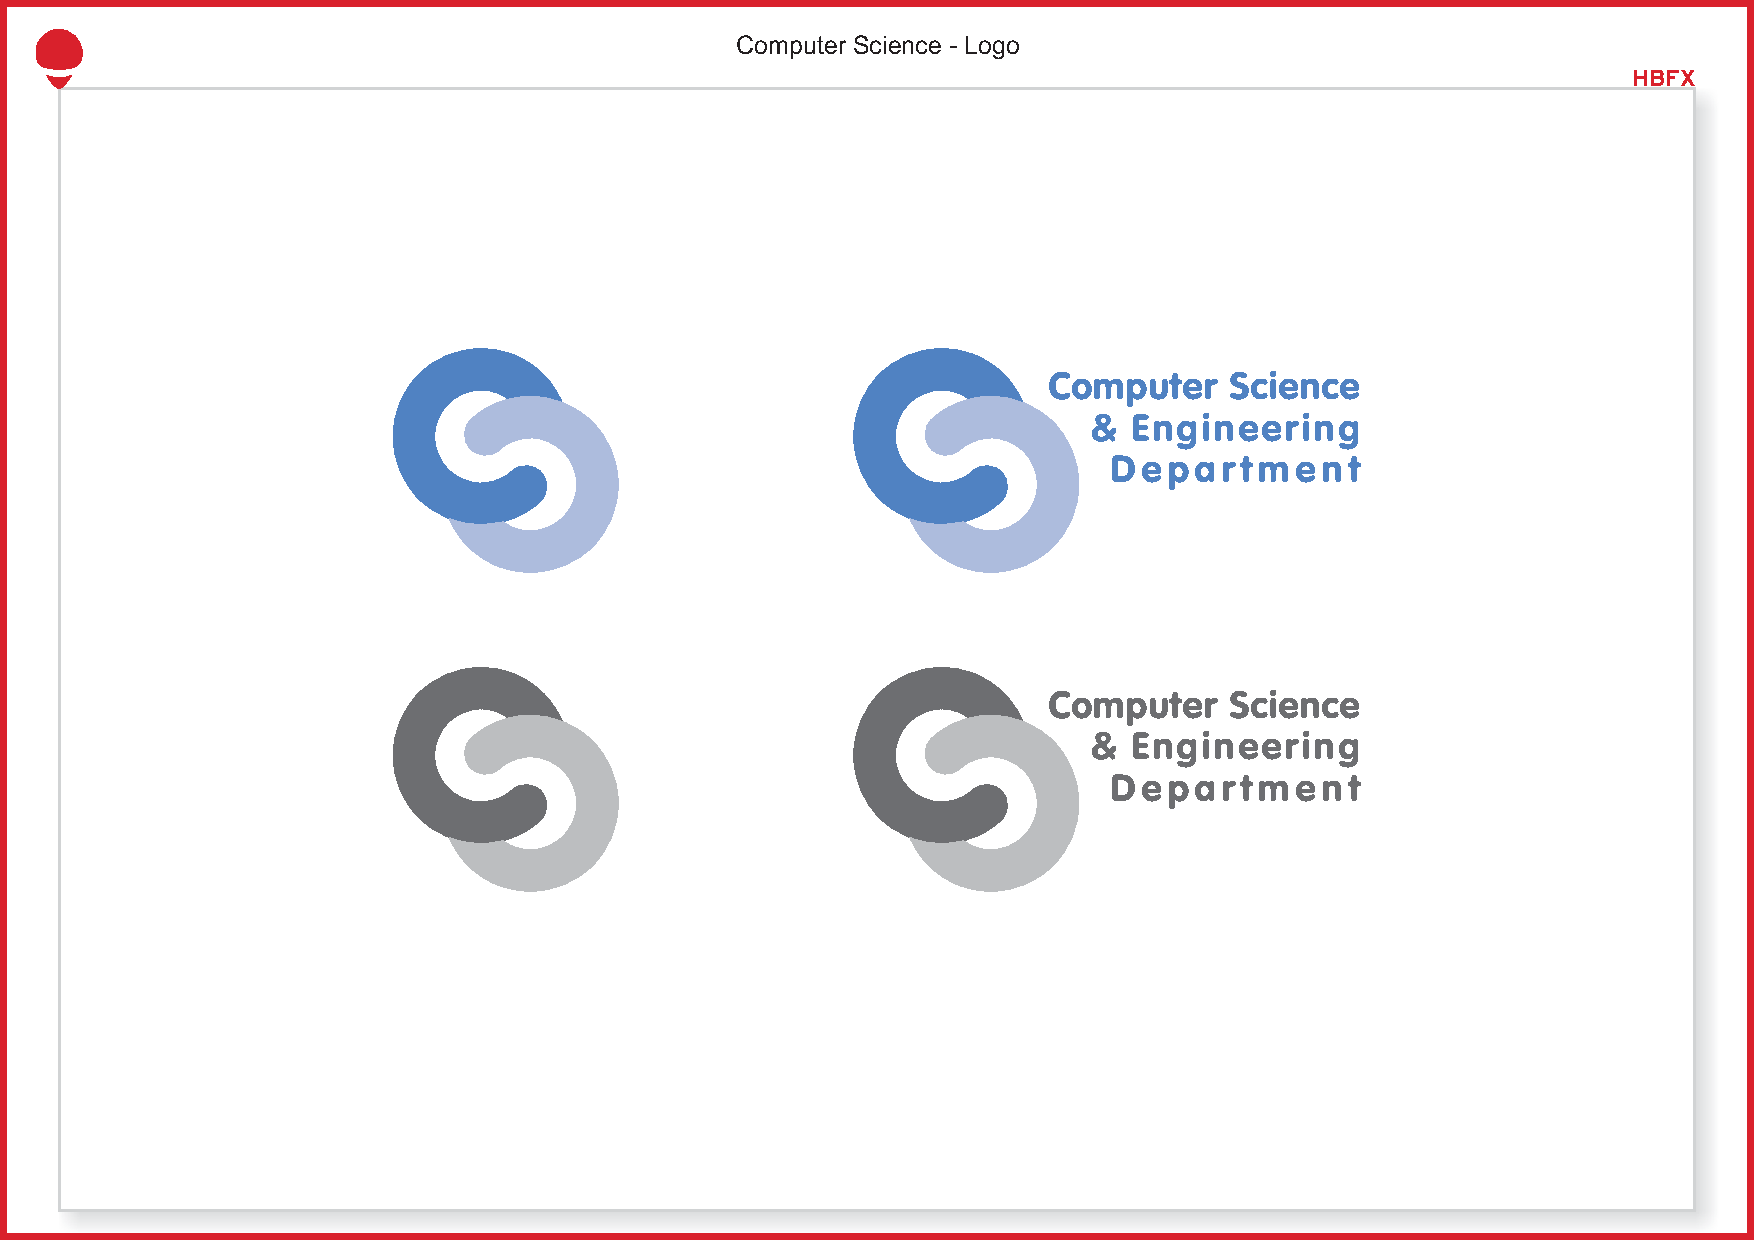
\includegraphics[scale=0.5,trim={14cm 11cm 2cm 5cm},clip=true]{pics/cs-logo.pdf}
\end{tabular}

\vspace{105pt}
{\Huge #2}\\                           % diploma project text
\vspace{40pt}
{\Large #3}\\ \vspace{0pt}  % project title
{\Large #4}\\                          % project subtitle
\vspace{40pt}
{\LARGE \Name}\\                   % student name
\end{center}
\vspace{60pt}
\begin{tabular*}{\textwidth}{@{\extracolsep{\fill}}p{6cm}r}
&{\large\textbf{#5}}\vspace{10pt}\\      % scientific advisor
&{\large \Advisor}                                    % advisor name
\end{tabular*}
\vspace{20pt}
\begin{center}
{\large\textbf{#6}}\\                                % bucharest
\vspace{0pt}
{\normalsize \Year}
\end{center}
\end{titlepage}
}

\newcommand{\frontPageRO}{\frontPage{\UniTextRO}{\DiplomaRO}{\ProjectTitleRO}{\ProjectSubtitleRO}{\AdvisorRO}{\BucRO}}
\newcommand{\frontPageEN}{\frontPage{\UniTextEN}{\DiplomaEN}{\ProjectTitleEN}{\ProjectSubtitleEN}{\AdvisorEN}{\BucEN}}

\linespread{1.15}
\setlength\parindent{0pt}
\setlength\parskip{.28cm}

%% Abstract macro
\newcommand{\AbstractPage}{
\begin{titlepage}
\textbf{\large SINOPSIS}\par
\AbstractRO\par\vfill
\textbf{\large ABSTRACT}\par
\AbstractEN \vfill
\end{titlepage}
}

%% Thank you macro
\newcommand{\ThanksPage}{
\begin{titlepage}
{\noindent \large\textbf{MULȚUMIRI}}\\
\Thanks
\end{titlepage}
}

%% Listing styles
\usepackage{listings}
\usepackage{xcolor}

\colorlet{punct}{red!60!black}
\definecolor{background}{HTML}{EEEEEE}
\definecolor{delim}{RGB}{20,105,176}
\colorlet{numb}{magenta!60!black}

\lstdefinelanguage{json}{
    basicstyle=\scriptsize,
    numbers=left,
    numberstyle=\scriptsize,
    stepnumber=1,
    numbersep=8pt,
    showstringspaces=false,
    breaklines=true,
    frame=lines,
    backgroundcolor=\color{background},
    literate=
     *{0}{{{\color{numb}0}}}{1}
      {1}{{{\color{numb}1}}}{1}
      {2}{{{\color{numb}2}}}{1}
      {3}{{{\color{numb}3}}}{1}
      {4}{{{\color{numb}4}}}{1}
      {5}{{{\color{numb}5}}}{1}
      {6}{{{\color{numb}6}}}{1}
      {7}{{{\color{numb}7}}}{1}
      {8}{{{\color{numb}8}}}{1}
      {9}{{{\color{numb}9}}}{1}
      {:}{{{\color{punct}{:}}}}{1}
      {,}{{{\color{punct}{,}}}}{1}
      {\{}{{{\color{delim}{\{}}}}{1}
      {\}}{{{\color{delim}{\}}}}}{1}
      {[}{{{\color{delim}{[}}}}{1}
      {]}{{{\color{delim}{]}}}}{1},
}


% Github Logo
\usepackage{fontawesome}

% hyphenation
\hyphenation{PostgreSQL}
\hyphenation{DigitalOcean}

%%%%%%%%%%%%%%%%%%%%%%%%%%%%%%%%%%%%%%%%%%%%%%%%%%   
%%
%%          End of template definitions
%%   
%%%%%%%%%%%%%%%%%%%%%%%%%%%%%%%%%%%%%%%%%%%%%%%%%%


%%% Puteți elimina aceste linii din lucrare, servesc numai pentru template.
\newcommand{\worktype}[1]{[\textit{#1}] }
\newcommand{\dezvoltare}{\worktype{Dezvoltare de produs}}
\newcommand{\cercetare}{\worktype{Cercetare}}
\newcommand{\ambele}{\worktype{Ambele}}
%%%

\addtocontents{toc}{\protect\thispagestyle{empty}}
%%
%%   Campurile de mai jos trebuie modificate de autor. Modificati doar continutul, nu si numele fiecarei definitii
%%
\newcommand{\ProjectTitleRO}{AcadNet.dev}
\newcommand{\ProjectSubtitleRO}{Platformă online pentru rezolvarea problemelor de informatică}
\newcommand{\ProjectTitleEN}{AcadNet.dev}
\newcommand{\ProjectSubtitleEN}{Online platform for solving computer science problems}
\newcommand{\Name}{Dimitrie David}
\newcommand{\Advisor}{Prof. Dr. Ing. Răzvan Victor Rughiniș }
\newcommand{\Year}{2023}

% Setări document
\title{Proiect de diplomă}
\author{\Name}
\date{\Year}

%%
%%   Campurile aferente rezumatului
%%
\newcommand{\AbstractRO}{Această lucrare prezintă \href{https://acadnet.dev}{AcadNet.dev}, o platformă online pentru rezolvarea de probleme de informatică. Platforma oferă un mediu de lucru complet, care permite utilizatorilor să creeze probleme, să le rezolve și să le evalueze automat. Platforma oferă și un mediu de lucru online, care permite utilizatorilor să rezolve problemele direct în browser, fără a fi nevoie să configureze un mediu de dezvoltare local.}

\newcommand{\AbstractEN}{This paper presents \href{https://acadnet.dev}{AcadNet.dev}, an online platform for solving programming problems. The platform offers a complete working environment, which allows users to create problems, solve them and automatically evaluate them. The platform also provides an online working environment, which allows users to solve problems directly in the browser, without the need to configure a local development environment.}

%%
%%   Campurile aferente paginii de multumiri
%%
\newcommand{\Thanks}{(opțional) Aici puteți introduce o secțiunea specială de mulțumiri / acknowledgments. }

\begin{document}

\frontPageRO
\frontPageEN

\begingroup
\linespread{1}
\tableofcontents
\endgroup

\AbstractPage

% Textul licentei incepe de aici 


% INRODUCTION
\chapter{Introduction}\pagestyle{fancy}
\section{Motivation and problem statement}
For the past half year, I was responsible for coordinating the development of problems for the Software Interoperability section of the \href{https://acadnet.ro/}{National Olympiad of Applied Informatics - Acadnet}. This section is different than the regular informatics olympiad, as it focuses more on the engineering side of informatics, rather than the theoretical side. The problems are more practical and require students to be more creative in order to solve them.

The problems are formulated as real life scenarios, where a code is given that should have a certain behavior, but it does not. The students have to find bugs in the code and fix them.

As of right now, there is no accessible methods for students to train for this olympiad. The only way for practicing is to solve the problems from the previous years, by downloading their statement and original source. There are no tests to check if the solution is correct. The students have to compile and run the code themselves, and check if the output is correct.

The platform's goal is to create an environment where students can train and prepare for the olympiad in a more efficient way. Moreover, we want to create an online workspace for students, where they can solve the problems directly in the browser. This allows us to get more creative with the engineering problems, as we can use more programming languages and configurations, without putting the students through the hassle of setting up a local development environment.

\section{Objectives}
During the last half year, I have been gathering insights on what the students and authors want from a platform like this. I have also been researching the available technologies, and I have been experimenting with different approaches. Based on this, the objectives of this project are defined as follows.

The objective of this project is to create a universal platform for solving engineering tasks. This should include the ability for authors to extend the platform and implement any new language that they want to write a problem in. In addition, the platform should give students the opportunity to solve the tasks directly in the browser, without requiring anything more than an account.
In terms of functionality, the platform should allow authors to create problems, and students to solve them. The platform should also provide a way to automatically evaluate the solutions, and give feedback to the students.

In terms of security, because the solutions will be evaluated by executing user-written code, the platform should be able to run the code in a sandboxed environment and prevent malicious code from being executed. The platform should also prevent students from cheating, by not allowing them to see the test cases, other users submissions, or the source code of the solutions.

The platform should be easily maintainable, and should be able to scale to a large number of users. It should use containerization to allow for easy deployment and scaling.

\section{Proposed solution and achieved results}
The core of the platform is a web application, which acts as the interface between the users and the platform. The web application is responsible for managing the users, problems, submissions, and for evaluating the submissions. In addition to this, the web application will also be a reverse proxy for online workspaces.

The web application is backed by a SQL database and an S3 file storage. The database is used to store the users, problems, submissions, and other metadata. The file storage is used to store the source code of the problems, and the submissions.

The web application is written in C\# using the .NET Core framework. The database is a PostgreSQL database, and the file storage is an S3 compatible storage, provided by DigitalOcean. The web application is deployed using Helm Charts on a Kubernetes cluster, also provided by DigitalOcean. The checker is written in Python and it acts as a sandbox manager that spawns a new container for each submission, and runs the tests inside the container. Like the checker, the workspace manager is also written in Python, and it is responsible for spawning new workspaces. Workspaces are Docker images based on a Visual Studio Code fork, that allows us to run the code directly in the browser.

The working platform can be found at \href{https://acadnet.dev}{AcadNet.dev} and the source code is open-source and available on Github inside the \href{https://github.com/acadnet-dev}{acadnet-dev} organization.


% PROPOSED SOLUTION
\chapter{System design and architecture}
\section{User journey}
\label{user-journey}
\begin{figure}[h]
	\centering
	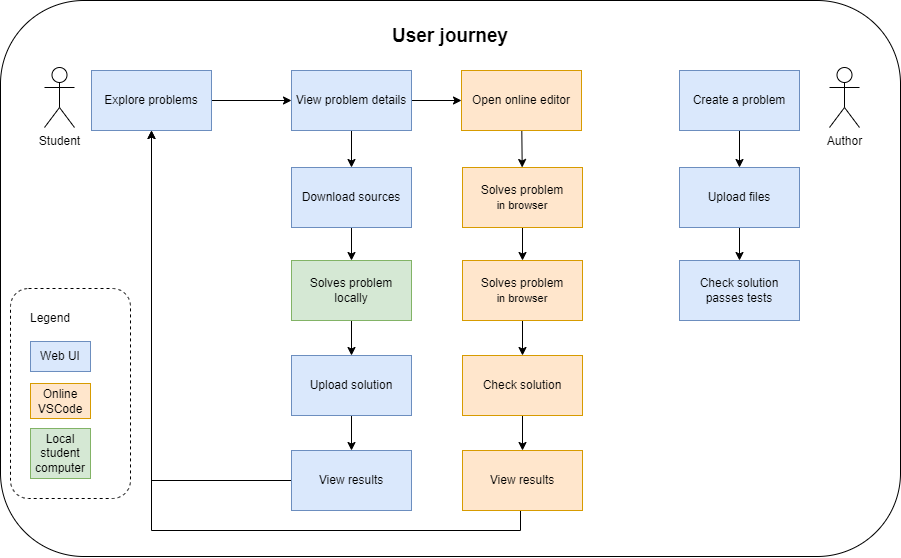
\includegraphics[width=\linewidth]{../photos/user-journey.png}
	\caption{User journey}
	\label{fig:user-journey}
\end{figure}

The platform's main actors are the users that want to learn and practice programming, by solving the problems available. The students can browse the problems, but in order to solve them, they have to create an account. After that, they can choose to solve the problems directly in the browser or they can download the source code and solve them locally. After they solve the problem, they can submit their solution for evaluation. The platform will automatically evaluate the solution, and give feedback to the them.

The other actors are the authors, who are responsible for creating the problems. The authors can create problems, and upload relevant files for the problem. These files include the statement, the source code of the problem, the test cases, and the solution.

\section{Architecture overview}
The architecture is composed of 3 main components: the web application, the checker, and the VSCode workspaces. The web application is the main component, and it is responsible for managing the users, problems, submissions, and for evaluating the submissions. The checker is responsible for evaluating the submissions, and the VSCode workspaces are used to allow users to solve the problems directly in the browser. The block diagram of the architecture can be seen in the figure below.

\begin{figure}[h]
	\centering
	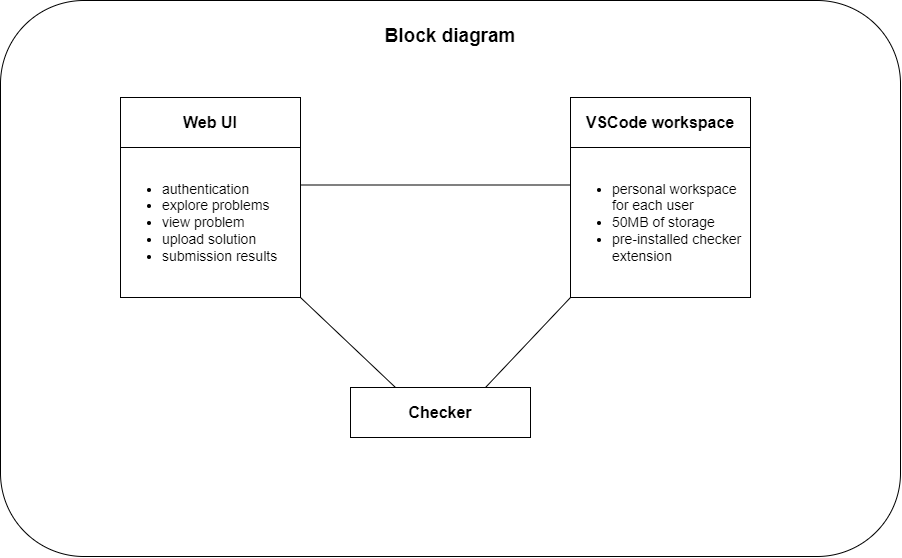
\includegraphics[width=\linewidth]{../photos/block-diagram.png}
	\caption{Software block diagram}
	\label{fig:software-architecture}
\end{figure}

\begin{table}[th]\small\linespread{1}
\caption{Component's responsibilities}
\label{tab:criterii}
\begin{tabular}{l >{\raggedright\arraybackslash}p{10cm} >{\raggedright\arraybackslash}p{0cm}}
\textbf{Component} & \textbf{Responsibilities} \\\hline
\textbf{Web App} & Manage users, problems and submissions; send submissions to the checker and present results; manage VSCode workspaces & \\
\hline
\textbf{Checker} & Test submissions by spawning a new sandbox in the K8s cluster and compare reference outputs with actual outputs & \\
\hline
\textbf{VSCode workspace} & Allow users to solve problems directly in the browser & \\
\hline
\end{tabular}
\end{table}

\newpage
\section{System components and interactions}
The web app is the brain of the platform. It is interacting with all the other components. With regards to the checker, the web app is responsible for receiving the submissions from the user or from the online workspace and to send them to the checker. While the checker is evaluating the submission, the web app constantly polls the checker for the updates and results. When the checker is done, the web app will receive the results and will update the submission with the status. On the other hand, when it comes to the interaction with the online workspaces, the web app is responsible for spawning new workspaces via the workspace manager and it acts as a HTTP and websocket proxy between the user's browser and the workspace.

\begin{figure}[h]
	\centering
	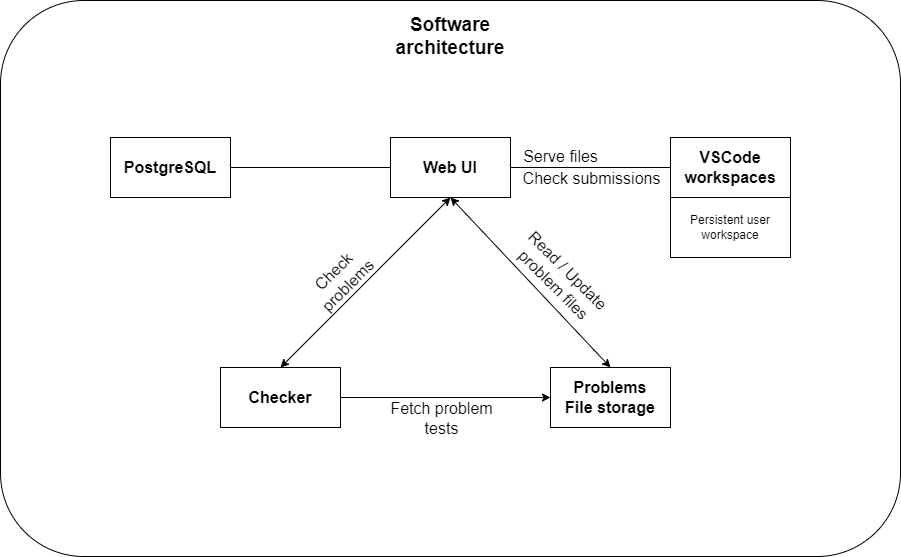
\includegraphics[width=\linewidth]{../photos/software-architecture.png}
	\caption{System components and their interactions}
	\label{fig:system-components}
\end{figure}

\subsection{SQL and file storage}
Other than the 3 main components, the architecture also includes a SQL database and an S3 file storage. The database is used to store the users, problems, submissions, and other metadata. The file storage is used to store the source code of the problems, and the submissions. The interactions between the components can be seen in Figure \ref{fig:system-components}. The web application is the only component that interacts with the database. The web application and the checker are the only components to interact with the file storage. The web application uses it to store the files uploaded by the authors, and the checker uses it to pull the test cases for the problem.


\section{Database design}
The database is designed using an ORM (Object Relational Mapper) called Entity Framework. This allows us to define the database schema using C\# classes, and because we are using a "code first" approach, the database tables and relations are created automatically, using migrations. The database schema can be seen in the figure below. 

\begin{figure}[h]
	\centering
	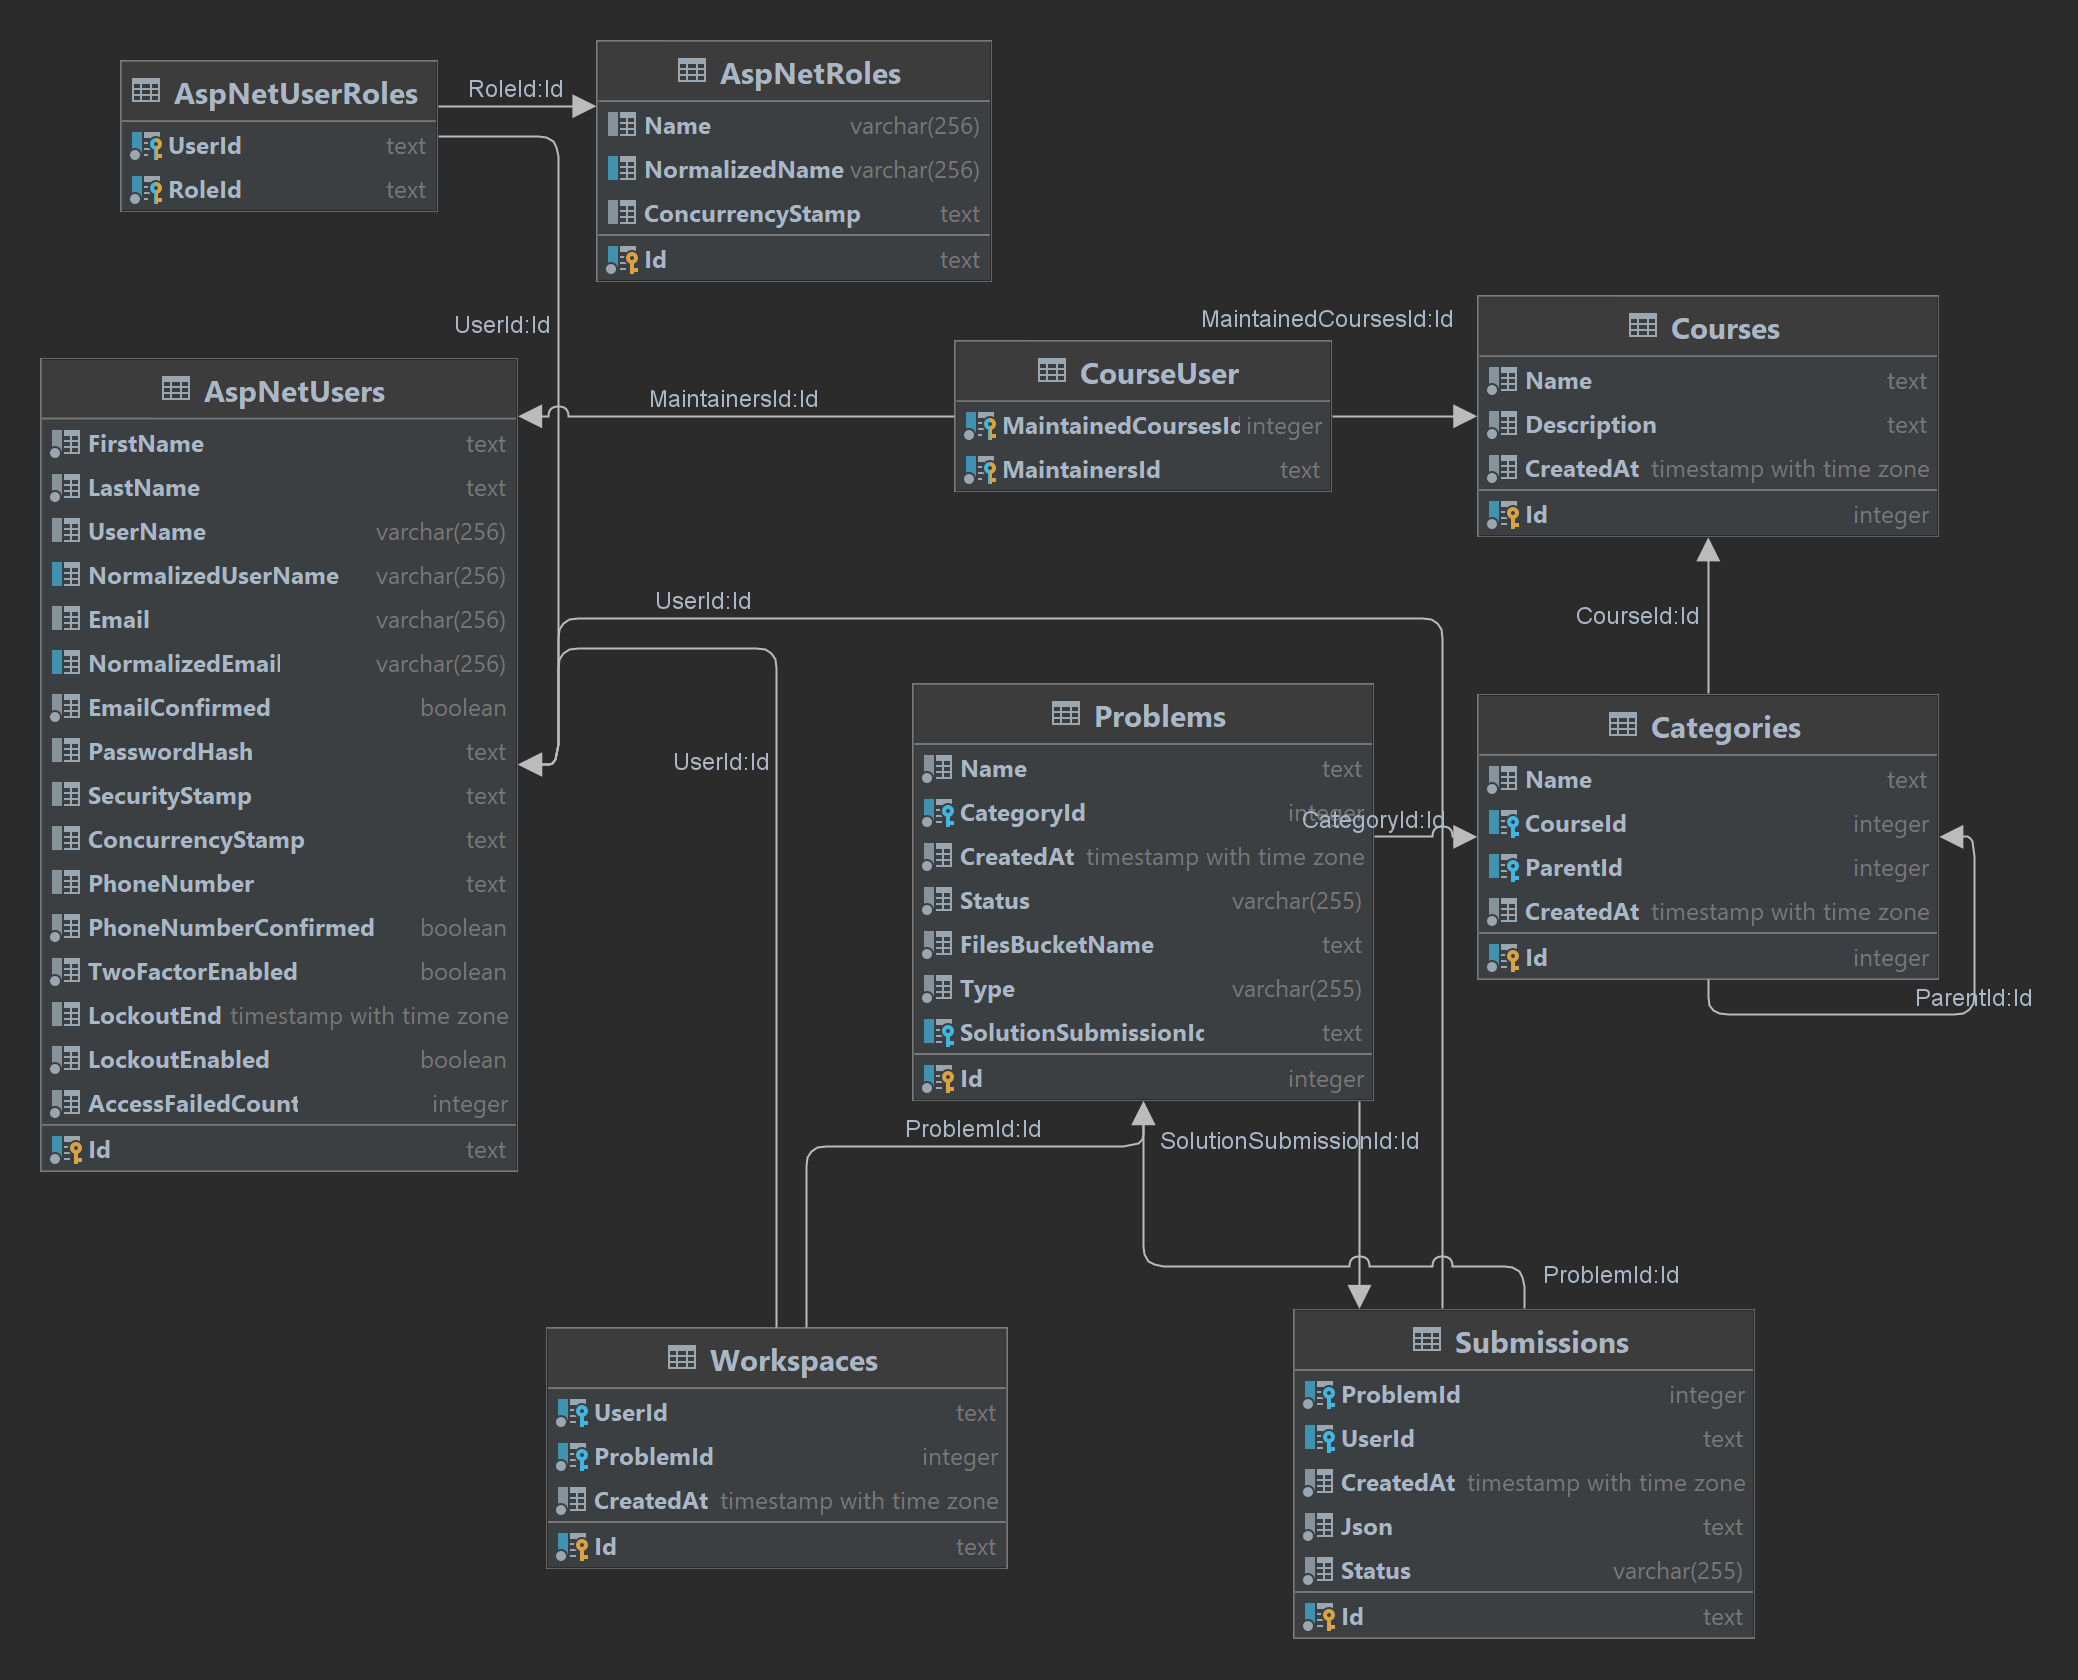
\includegraphics[width=\linewidth]{pics/database-schema.png}
	\caption{Database schema diagram}
	\label{fig:database-schema}
\end{figure}

As we can see in Figure \ref{fig:database-schema}, the database is composed of multiple tables. Some of them are automatically generated by the .NET Identity Framework that handles authentication.

Below is a description of each table and its purpose.

\newpage
\subsection{Users and roles}
\label{users-and-roles}
\begin{itemize}
	\item \textbf{AspNetUsers} - stores the users that have an account on the platform. The users can be either students or authors.
	\item \textbf{AspNetRoles} - stores the roles available on the platform; currently, there are only 2 roles: student and author.
	\item \textbf{AspNetUserRoles} - because the relation between users and roles is many to many, this table is needed to store what roles each user has.
\end{itemize}

\subsection{Problem hierarchy}
The problems are organized in a tree-like structure. As the root there are the courses that have a name and a description. Each course has multiple categories, and each category can have as children other categories or problems. An example of the hierarchycal structure is shown in Figure \ref{fig:problem-hierarchy}.

\begin{figure}[h]
	\centering
	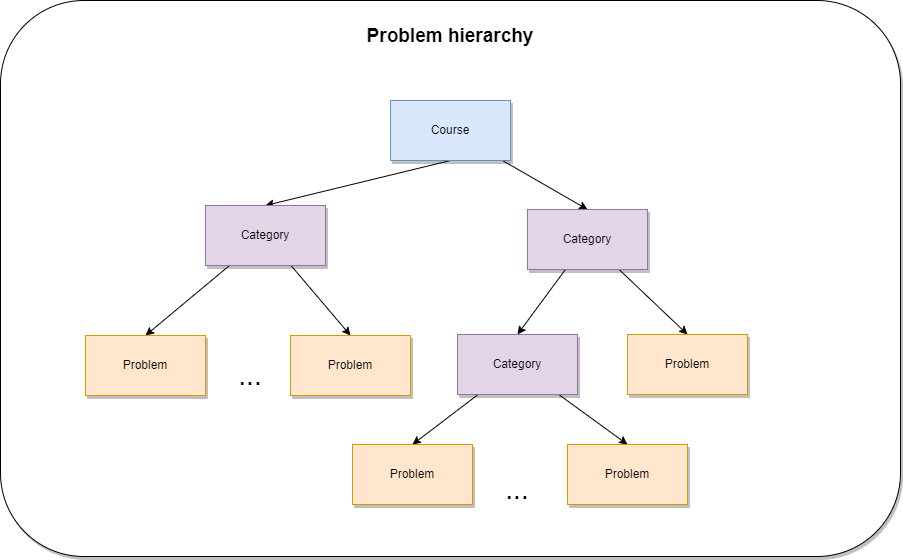
\includegraphics[width=\linewidth]{../photos/problem-hierarchy.png}
	\caption{Problem hierarchy}
	\label{fig:problem-hierarchy}
\end{figure}

\begin{itemize}
	\item \textbf{Courses} - stores the courses available on the platform.
	\item \textbf{CourseUser} - a course can have maintainers; this table stores the relation between the courses and the users that are maintainers.
	\item \textbf{Categories} - stores the categories available on the platform; each category has a course and may have a parent category.
	\item \textbf{Problems} - stores the problems available on the platform; each problem belongs to a category. Also, the problem stores the bucket id of the file storage where the problem's files are stored.
\end{itemize}

\subsection{Submissions and workspaces}

\begin{itemize}
	\item \textbf{Submissions} - stores the submissions made by the users; each submission has a problem and a user.
	\item \textbf{Workspaces} - stores the workspaces available on the platform; each workspace has a problem and a user.
\end{itemize}

% IMPLEMENTATION DETAILS
\chapter{Implementation details}
\label{implementation-details}
All the code for the platform and all its components is available on Github inside the \href{https://github.com/acadnet-dev}{acadnet-dev} organization.

\section{Web application \href{https://github.com/acadnet-dev/web}{\faicon{github} Repository}}
The web application is the main component of the platform. It is responsible for managing the users, problems, submissions, and for evaluating the submissions. In addition to this, the web application acts as a reverse proxy for the online workspaces. The web application is written in C\# using the .NET Core framework. It is using the MVC (Model-View-Controller) pattern, and it is using an ORM (Object Relational Mapper) called Entity Framework to interact with the database. The web application is deployed as a Docker image using multi-stage builds. The Docker image is deployed on a Kubernetes cluster using Helm Charts. The web application is composed of multiple components, which are described below.

\subsection{Controllers}
The controllers are the components that handle the HTTP requests. They receive a request from the user and process it by calling different services and interacting with other components so that it returns a response. The platform has multiple controllers, each acting in its own domain. The controllers are described below.

\textbf{AuthController}
It handles all the actions related to user authentication and authorization. It is responsible for registering new users, logging in existing users, and managing the user's roles.

Registering users and logging in users is done via external authentication providers. Currently, the platform only supports Google authentication, but it can be easily extended to support other providers. Support for other popular external providers is already implemented in the .NET framework.

\textbf{CoursesController}
It handles all the actions related to courses like creating new courses. This action can be done only by users that have the author role. It also handles creating categories and listing the hierarchycal structure of the courses and categories so that users can browse them.

\newpage
\textbf{ProblemsController}
This controller handles creating new problems, showing the problem's statement, and evaluating the submissions. Problems can only be created if the user is a maintainer of the course.

Submitting a solution is done by uploading a file with the solution's source code. The file is sent to the checker. There is also a `GET` endpoint that returns the submission's status. This endpoint is called periodically by the frontend to check if the submission is done.

\textbf{WorkspaceController}
This controller is responsible for managing the online workspaces. It handles creating new workspaces, and sets the environment for the proxy to connect to the workspace. More details about the proxy and how the workspaces are accessed by the user's browser can be found in Section \ref{workspaces-proxy}.

\subsection{UI}
The UI is built using the Razor Pages framework. It is created based on a template from \href{https://themeforest.net/}{Theme Forest}.
In terms of technologies, the UI uses SASS, jQuery, and Bootstrap. The UI is responsive and it works on both desktop and mobile devices.

Some of the interesting elements that the UI has are described below.

\textbf{Problem statement}
The problem author's are required to upload a Markdown file with the problem's statement. The UI is using the \href{https://github.com/xoofx/markdig}{Markdig} library to convert the Markdown file to HTML. The HTML is then rendered in the browser using custom CSS styles for the different elements in Markdown.

\textbf{File upload}
The file upload input is a custom component that is using the \href{https://pqina.nl/filepond/}{FilePond} library. This library is responsible for creating a responsive and dynamic file upload input. It lets authors upload multiple files at once and remove already uploaded files. It also has a drag and drop feature, and it can be easily extended to support other features like file validation, file preview, and image editing. 

\begin{figure}[h]
	\centering
	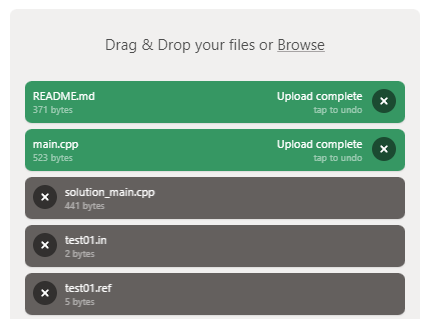
\includegraphics[width=230px]{./pics/file-uploader.png}
	\caption{File upload component}
	\label{fig:file-upload}
\end{figure}

\newpage
\subsection{Services}
The services are the components that handle the business logic of the platform. They are used by the controllers to process requests. They are responsible for interacting with the database and the file storage. Services are a pair made of an interface describing the available methods and a class implementing the interface. Services are using a dependency injection mechanism to be injected into the controllers and other services. The functionality of each service is described below.

\textbf{FileService}
This service is responsible for interacting with the file storage. It is used to create buckets\protect\footnotemark{} and upload and download files from the file storage.
\footnotetext{A bucket is a collection of files in an S3 compatible storage}

\textbf{ProblemService}
This service handles all the actions regarding problems. It is implemented using the Factory Pattern, because the problems can be written in different languages and have different methods of evaluation and initialization. Currently, the platform implements only one type of problem with one file source code of C++ and tests that are based on finding differences between the reference output and the actual output. But it can be easily extended to support other types of problems, written in other languages, and with other methods of evaluation like asserting the execution time or the memory usage.

Some of the methods that needs to be implemented for each type of problem are described below.

\begin{itemize}
	\item creating a problem
	\item getting a problem by id
	\item getting a problem's statement and converting it from Markdown to HTML
	\item get the sources of a problem to be downloaded by the user
	\item get the test cases of a problem so that they can be sent to the checker
	\item creating and updating a submission
	\item getting the necessary files to initialize a workspace
\end{itemize}

\textbf{CheckerService}
This service is responsible for interacting with the checker. It is used to create submissions and to get the status of a submission.

\textbf{WorkspaceService}
This service is responsible for interacting with the workspace manager. It is used to create workspaces and to get the URL of a workspace for the reverse proxy.

\subsection{Workspaces Proxy} \label{workspaces-proxy}
The workspaces reverse proxy is a component that acts as an intermediate between the user's browser and the workspace. It is responsible for receiving user requests for the workspace and redirecting them to the appropriate workspace container. It also handles the websocket connections between the user's browser and the workspace container.

The proxy is written as a middleware in .NET Core and it is part of the web application. Because of this, it is very easy to check if the user is authenticated and authorized to access the workspace, because the authentication cookies are already in the user's browser and are transmitted with each request. 

\section{SQL database}
The SQL database is a PostgreSQL database. It is deployed as a managed service on DigitalOcean. The database is used to store the users, problems, submissions, and other metadata. The database schema can be seen in Figure \ref{fig:database-schema}. The web application is the only component that interacts with the database. It is controlled using Entity Framework, which is an ORM (Object Relational Mapper) that allows us to define the database schema using C\# classes. The database tables and relations are defined in a "code-first" approach, which means that the tables and relations are created by the ORM by translating the C\# classes and relationship between them to tables and keys.

Each modification to the database schema is handled by migrations. Migrations are C\# classes that describe the changes that need to be made to the database schema. The migrations are created automatically by the ORM, and they are applied automatically when the application starts. This allows for easy modifications on the database schema without having to manually create the tables and relations.

\section{File storage}
The platform needs a distributed storage method for the files uploaded by the authors and the submissions made by the users. An S3 compatible storage is a good solution for this, because it is easy to use and it is scalable. For this project, when developing, we are running a local S3 compatible storage using \href{https://min.io/}{MinIO}. For production, we are using a managed S3 compatible storage provided by DigitalOcean called \href{https://www.digitalocean.com/products/spaces/}{Spaces}.

The storage is accessed using Amazon's S3 C\# SDK. The SDK is used to create buckets, upload and download files, and list files in a bucket. The buckets are created automatically by the web application when a new problem is created. The bucket's name is a UUID and the files are uploaded with specific names, defined by the problem type.

\newpage
For example, for the C++ problems, the files uploaded need to have to respect this naming convention:

\begin{itemize}
	\item \textbf{main.cpp} - the source code of the problem
	\item \textbf{soltion\_main.cpp} - the source code of the solution
	\item \textbf{README.md} - the statement
	\item \textbf{test0.in} - the first test case
	\item \textbf{test0.ref} - the first test case's reference output
	\item \textbf{test1.in} - the second test case
	\item \textbf{test1.ref} - the second test case's reference output
	\item \textbf{...}
\end{itemize}

\section{Checker \href{https://github.com/acadnet-dev/checker}{\faicon{github} Repository}}
The checker is the component of the platform that handles the evaluation of the submissions. It is written in Python and it is exposed as a simple REST API. The checker is deployed as a Docker image on the Kubernetes cluster. The checker is composed of multiple components, which are described below.

\subsection{API}
The API is built using the \href{https://fastapi.tiangolo.com/}{FastAPI} framework. It is a simple REST API that exposes 2 endpoints: one for creating a new submission, and one for getting the status of a submission. The API is responsible for receiving the submission from the web application and for sending the results back to the web application.

The API endpoints are described below.

\textbf{POST /submission/create}
\begin{description}
	\item[Query parameters]\
		\begin{itemize}
			\item \textbf{type} - the type of the problem
			\item \textbf{bucket} - the bucket id where the problem's files are stored
		\end{itemize}
	\item[Request body]\
		\begin{itemize}
			\item \textbf{file} - the file with the source code of the submission as a multipart form data
		\end{itemize}
	\item[Response body]\
		\begin{itemize}
			\item \textbf{submission\_id} - the id of the newly created submission
		\end{itemize}
\end{description}

\newpage
\textbf{GET /submission/status}
\begin{description}
	\item[Query parameters]\
		\begin{itemize}
			\item \textbf{submission\_id} - the id of the submission
		\end{itemize}
	\item[Response body]\
		\begin{itemize}
			\item \textbf{status} - the status of the submission
		\end{itemize}
\end{description}

An example of a submission status for a C++ problem can be seen in the appendix \ref{anexa:cod:json-submission}. Important things to be noted are the presence of the compilation status, the expected and actual results for each test case and all the logs from the sandbox.

\subsection{Sandbox adapter}
The purpose of the sandbox adapter is to communicate with the Kubernetes cluster and with the sandbox itself, for things like creating the sandbox, uploading files to the sandbox, running commands inside the sandbox or purging the sandbox after the submission is evaluated.

When creating a submission, the actual thing that happens is that a new sandbox is launched so that the code can be executed inside it. The sandbox is a Docker container that is launched on the Kubernetes cluster. The sandbox is controlled with the \href{https://github.com/kubernetes-client/python}{Python Kubernetes client}. The launched sandbox depends on the type of problem that is being evaluated. This way we can have different types of problems, written in different languages, and with different methods of evaluation and the sandbox will have all the resources needed to evaluate the submission.

The interactions between the checker and other components can be seen in Figure \ref{fig:checker-interactions}.
\begin{figure}[h]
	\centering
	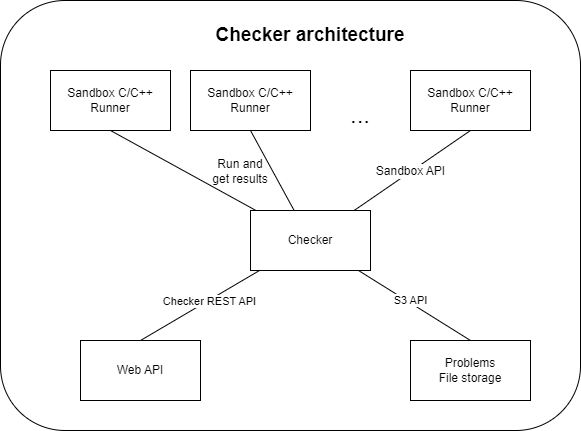
\includegraphics[width=300px]{../photos/checker-architecture.png}
	\caption{Checker interactions}
	\label{fig:checker-interactions}
\end{figure} 


\subsection{File manager}
All the files that come to the checker, being them received from the web application or downloaded from the file storage, are stored in a temporary directory. The file manager is responsible for managing the files in this directory. It is responsible for creating the directory, uploading files to the directory and deleting it when the submission is evaluated.

\subsection{Submission factory}
The submission factory is responsible for creating the submission object, based on the problem type. The implementation of the submission object is different for each type of problem. It needs to know stuff like what commands to run to build the code, how do the tests look, how to run them and how to compare the results. Currently, the platform only supports one type of problem, but it can be easily extended to support other types as well.

\subsection{Workflow for C++ problems}
\begin{enumerate}
	\item The checker receives a new submission from the web application via the API.
	\item The checker stores the submitted file in a temporary directory.
	\item Based on the problem type, the checker creates a new submission object.
	\item The submission object fetches all the necessary files from the S3 file storage.
	\item The sandbox adapter creates a new sandbox container on the Kubernetes cluster.
	\item The sandbox adapter uploads all the necessary files to the sandbox.
	\item The sandbox adapter runs the build command inside the sandbox.
	\item The sandbox adapter iterates through all the test cases and runs them inside the sandbox.
	\item The sandbox adapter compares the actual output with the reference output and stores the results.
	\item The sandbox adapter deletes the sandbox.
\end{enumerate}


\subsection{Global status object}
Each submission is ran in a background thread. The status is a global object that is updated by the sandbox adapter as it progresses through the workflow. When the API receives a request for the status of a submission, it returns the status object.

\section{Sandbox image \href{https://github.com/acadnet-dev/sandbox-cpp}{\faicon{github} Repository}}
All the sandbox images are running a Python FastAPI server that is used by the sandbox adapter to communicate with the sandbox.
Each sandbox image is created specifically for each problem type. Currently, the only sandbox image available is for C++ problems.
The image is based on the \href{https://hub.docker.com/_/gcc}{GCC Docker image} and has Python installed and all the dependencies for the FastAPI server.
Then the image is pushed to the Docker registry and it is deployed on the Kubernetes cluster via the sandbox adapter.

The endpoints of the FastAPI server are described below.

\textbf{POST /upload\_file}
\begin{description}
	\item[Request body]\
		\begin{itemize}
			\item \textbf{file} - the file to be uploaded; all the files are uploaded in the same directory
		\end{itemize}
	\item[Response status]\
		\begin{itemize}
			\item \textbf{200} - the file was uploaded successfully
			\item \textbf{other} - an error occurred
		\end{itemize}
\end{description}


\textbf{POST /run}\\
This endpoint is used to run commands on the sandbox and get the output. For example, it is used to run the build command and to run the tests.
\begin{description}
	\item[Request body]\
		\begin{itemize}
			\item \textbf{cmd} - the command to be run inside the sandbox
		\end{itemize}
	\item[Response body]\
		\begin{itemize}
			\item \textbf{stdout} - the standard output of the command
			\item \textbf{stderr} - the standard error of the command
			\item \textbf{returncode} - the return code of the command
		\end{itemize}
\end{description}

\newpage
\section{VSCode workspaces manager \href{https://github.com/acadnet-dev/workspaces}{\faicon{github} Repository}}
The VSCode workspaces manager is a component that is responsible for spawning new workspaces. It is written in Python and it is exposed as a simple REST API. The workspaces manager is deployed as a Docker image on the Kubernetes cluster. This manager is very similar to the checker, but it is much simpler. A workspace is unique for each user and problem.

It is responsible for receiving the request for a new workspace from the web application, and for spawning a new workspace container on the Kubernetes cluster. The workspace container is a Docker image based on a Visual Studio Code fork that allows us to run VS Code directly in the browser.

The workflow of creating a new workspace is described below.
\begin{enumerate}
	\item The users requests a new workspace from the web application by clicking a button.
	\item The web application creates the workspace object in the database and sends a request to the workspaces manager.
	\item The workspaces manager checks if the workspace already exists. If it does, it returns the internal IP of the workspace pod.
	\item If the workspace does not exist, the workspaces manager creates a new workspace pod on the Kubernetes cluster.
	\item The workspaces manager copies the necessary files to the workspace pod.
	\item The workspaces manager returns the internal IP of the workspace pod.
	\item The web application proxies the user's browser to the workspace pod.
\end{enumerate}

The endpoints of the workspaces manager are described below.

\textbf{POST /workspace/create}
\begin{description}
	\item[Request body]\
		\begin{itemize}
			\item \textbf{id} - the id of the workspace
			\item \textbf{problem\_name} - the name of the problem
			\item \textbf{files} - the files that need to be copied to the workspace
		\end{itemize}
	\item[Response body]\
		\begin{itemize}
			\item \textbf{endpoint} - the internal IP of the workspace pod
		\end{itemize}
\end{description}

\textbf{POST /workspace/get}
\begin{description}
	\item[Request body]\
		\begin{itemize}
			\item \textbf{id} - the id of the workspace
		\end{itemize}
	\item[Response body]\
		\begin{itemize}
			\item \textbf{endpoint} - the internal IP of the workspace pod
		\end{itemize}
\end{description}

\section{VSCode online image \href{https://github.com/acadnet-dev/vscode-server}{\faicon{github} Repository}}
As mentioned above, the workspace image is a web server that serves Visual Studio Code in the browser via HTTP requests and web sockets. The image is based on a fork of Visual Studio Code called \href{https://github.com/gitpod-io/openvscode-server}{Gitpod OpenVSCode Server} that allows us to run VS Code in the browser. The image is pushed to the Docker registry and it is deployed on the Kubernetes cluster via the workspaces manager.

The platform has its own fork of the Gitpod OpenVSCode Server, because we needed to make some changes to the code to make it work with our platform, like adding the checker extension. The fork can be seen here \href{https://github.com/acadnet-dev/vscode-server}{acadnet-dev/vscode-server}.

\section{VSCode checker extension \href{https://github.com/acadnet-dev/vscode-checker-extension}{\faicon{github} Repository}}

\begin{figure}[h]
	\centering
	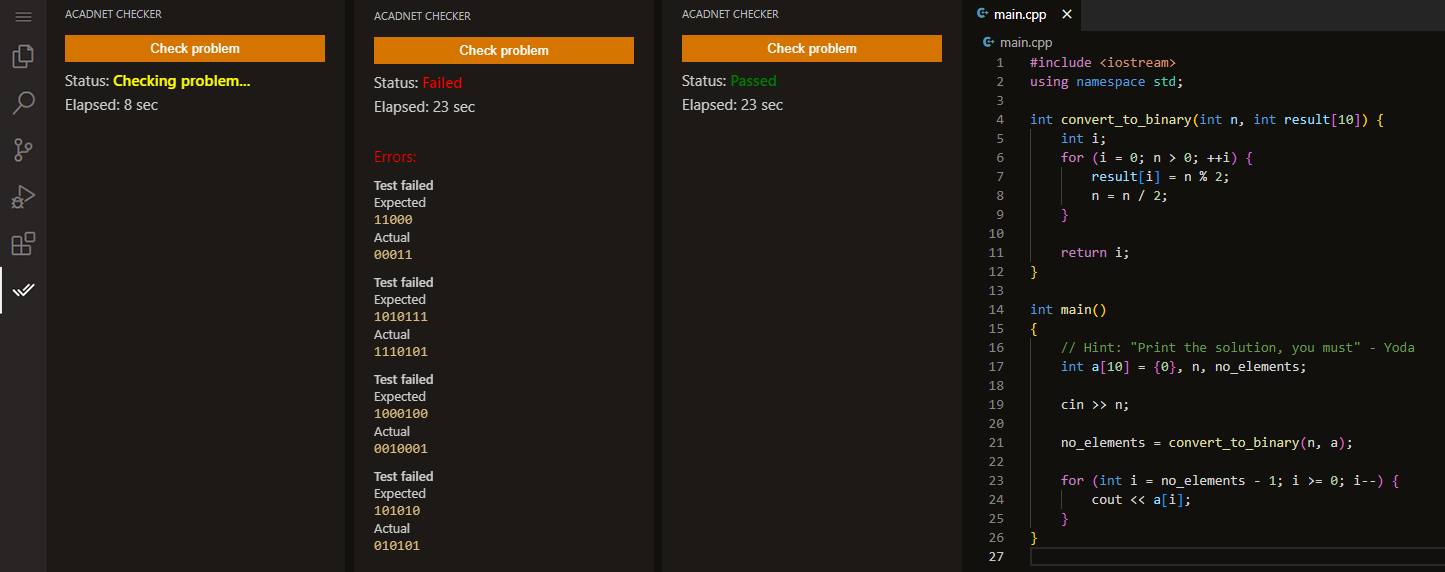
\includegraphics[width=\linewidth]{./pics/checker-extension.png}
	\caption{Checker extension example}
	\label{fig:checker-extension}
\end{figure}

The chceker extension is a custom made extension for Visual Studio Code that is created specifically to be run in the browser. It is written in TypeScript and it is composed of a frontend and a backend. The backend is responsible for communicating with the checker and the frontend is responsible for displaying the results to the user. The frontend is a sidebar panel that is displayed when the user clicks the extension's icon. The extension is written using the \href{https://code.visualstudio.com/api}{VS Code Extension API}. The backend uses fetch API to communicate with the web app for submitting solutions for the problem and polling for the results. The frontend uses plain HTML, JS and CSS to display the results.

The extension is installed compiled as a `.vsix' file and served as a \href{https://github.com/acadnet-dev/vscode-checker-extension/releases}{Github Release} in the repository. The workspace image pulls the extension and installs it. The extension is automatically enabled when the workspace is created.


% FEATURES AND FUNCTIONALITIES
\chapter{Features and functionalities}
\section{Main page}
The main page is the first page that the user sees when accessing the platform. It is a simple page that contains an incentive for the user to create an account and a list of the available courses. 

\begin{figure}[h]
	\centering
	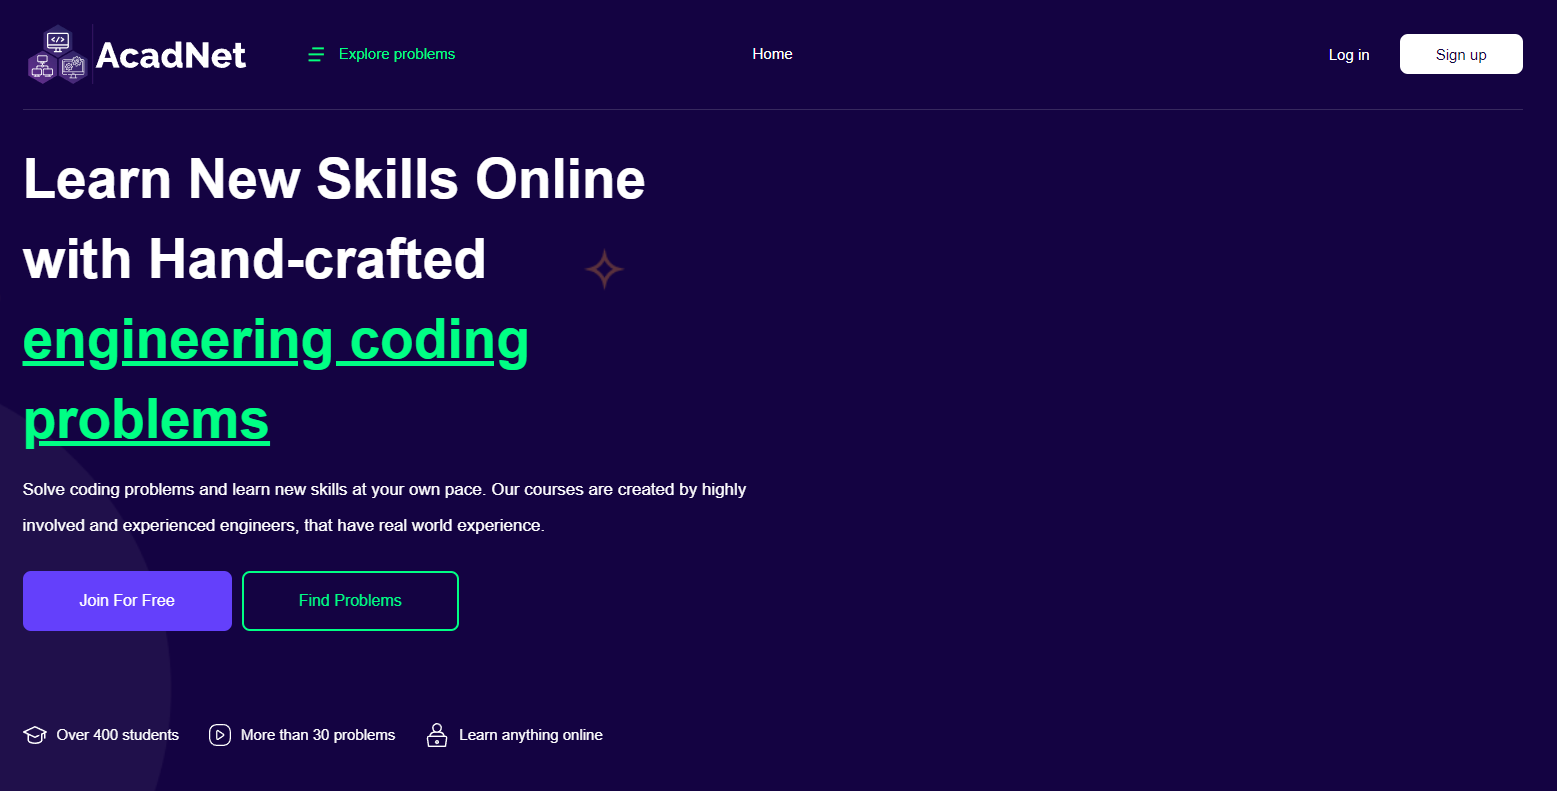
\includegraphics[width=300px]{./pics/front-page.png}
	\caption{Main page}
	\label{fig:main-page}
\end{figure}

\section{User authentication}
The users can register and log in using their Google account. This is done via the Google OAuth2 authentication provider.

\begin{figure}[h]
	\centering
	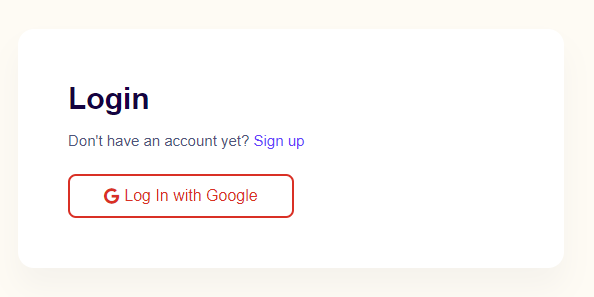
\includegraphics[width=300px]{./pics/login.png}
	\caption{Login page}
	\label{fig:login-page}
\end{figure}

\section{Problem browsing}
As a student, the user can browse the problems by course and category.

\begin{figure}[h]
	\centering
	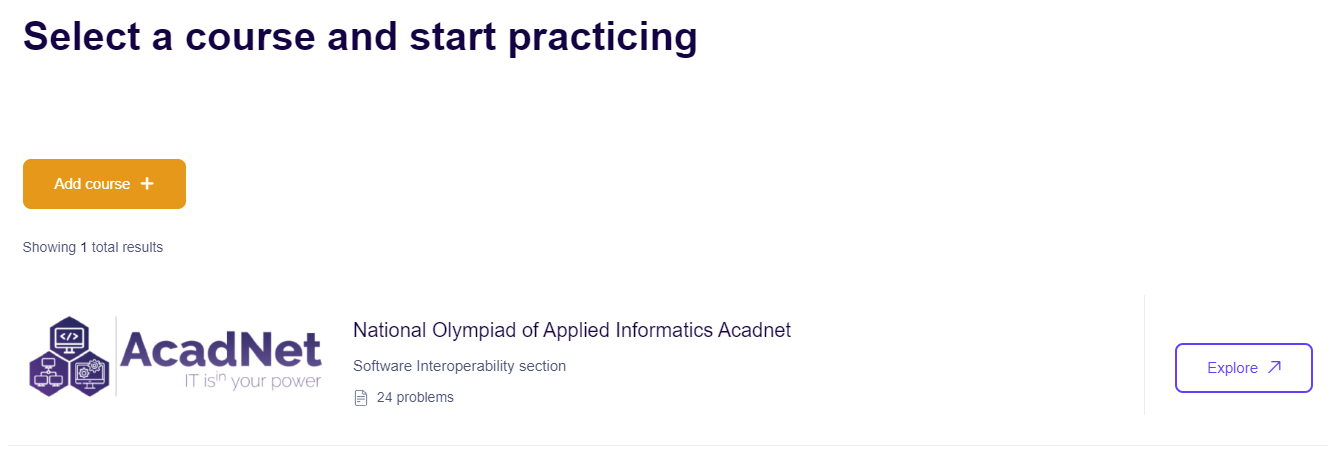
\includegraphics[width=\linewidth]{./pics/course.png}
	\caption{Course list}
	\label{fig:course}
\end{figure}

After selecting a course, the user can see the categories and problems in each category. In the figure below, the problems in category '9-10' are shown.

\begin{figure}[h]
	\centering
	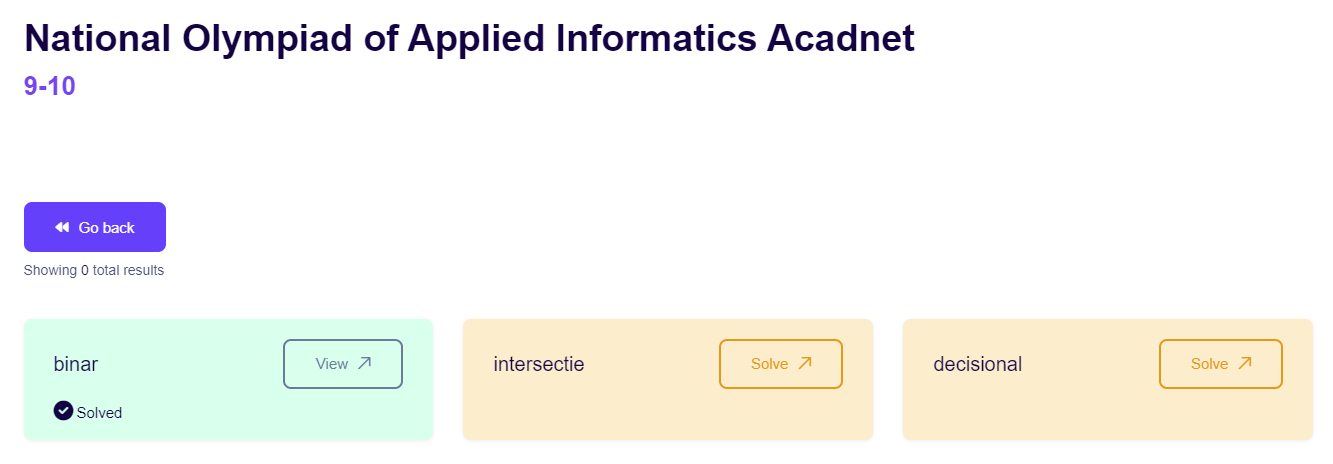
\includegraphics[width=\linewidth]{./pics/problem-list.png}
	\caption{Problem list}
	\label{fig:problem-list}
\end{figure}

\newpage
\section{Problem creation}
A problem can be created only by course maintainers. After the problem is created, its status is 'Incomplete' until the author uploads the necessary files and the solution passes all the tests. After that, the problem's status is 'Ready' and it can be solved by the students.

\begin{figure}[h]
	\centering
	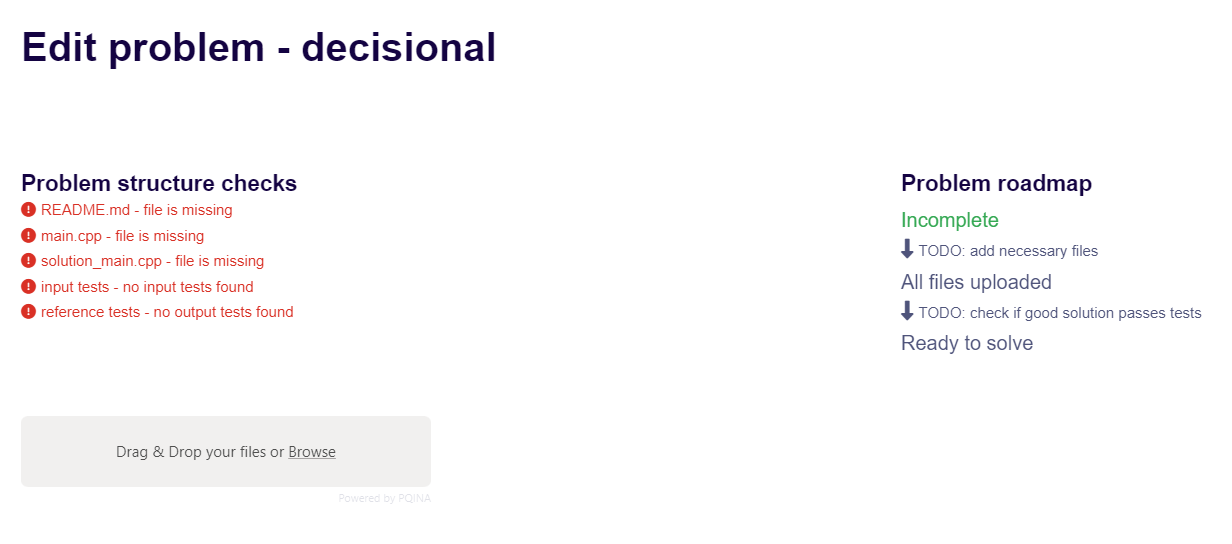
\includegraphics[width=\linewidth]{./pics/empty-problem.png}
	\caption{Problem editing}
	\label{fig:problem-editing}
\end{figure}

This is how a maintainer sees the problems in a category. In the figure below, we can see that the problem 'intersectie' is 'Ready' and the problem 'decisional' is 'Incomplete' in the category '9-10'.

\begin{figure}[h]
	\centering
	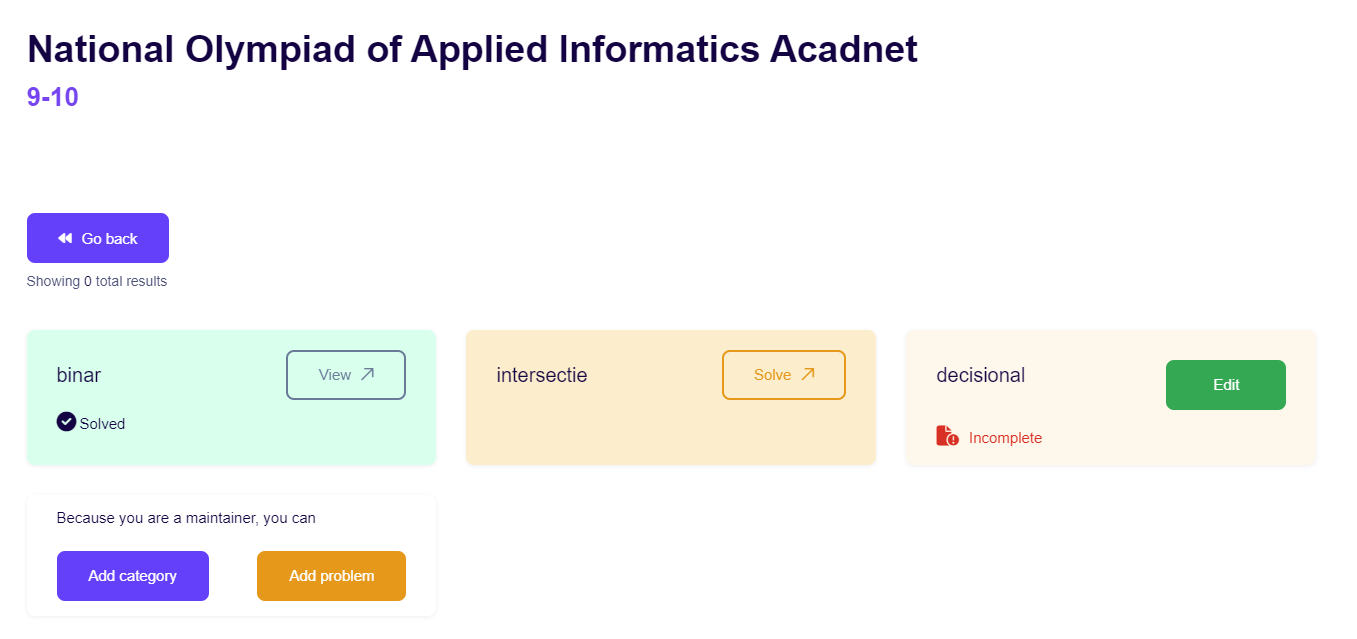
\includegraphics[width=\linewidth]{./pics/maintainer-problem-list.png}
	\caption{Maintainer problem list}
	\label{fig:maintainer-problem-list}
\end{figure}

\newpage
\section{Problem solving}
When a user chooses a problem to solve, he is shown the page in Figure \ref{fig:problem-solving}. The page contains the problem's statement, a button to download the sources, a file uploader for the solution and a button to luanch the online workspace. 
\begin{figure}[h]
	\centering
	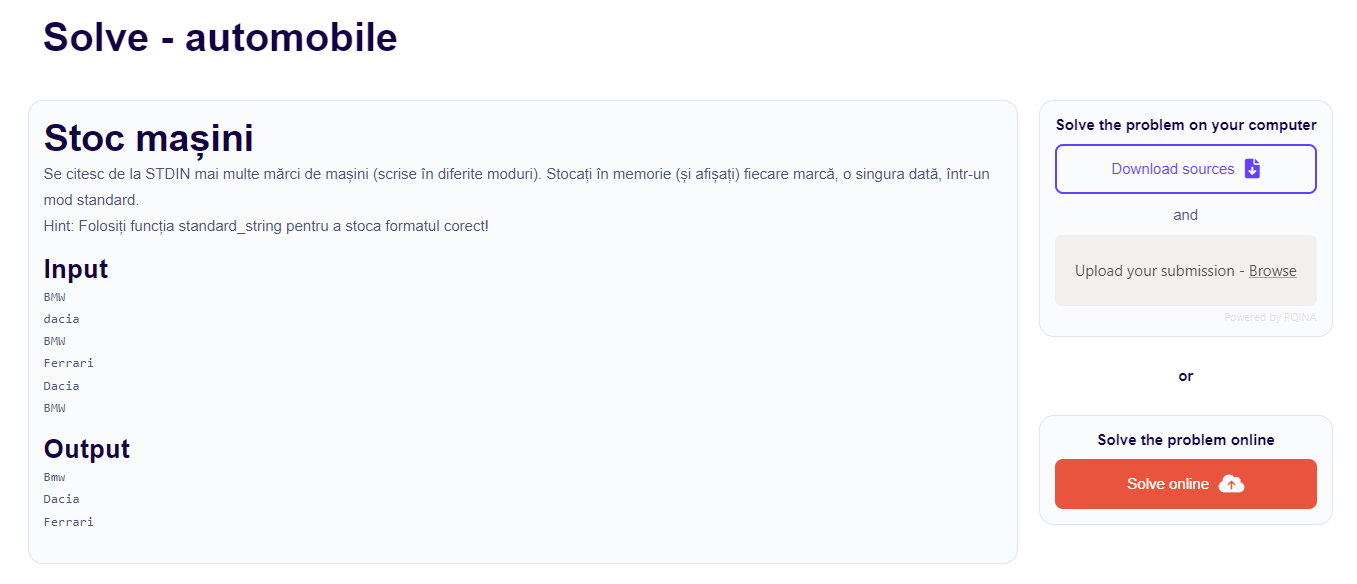
\includegraphics[width=\linewidth]{./pics/solve.png}
	\caption{Problem solving}
	\label{fig:problem-solving}
\end{figure}

\section{Submission evaluation}
The user can evaluate the submission directly in the problem solving page. He can upload the solution and see the status of the submission. In the figure below, we can see the process of submitting a solution.

\begin{figure}[h]
	\centering
	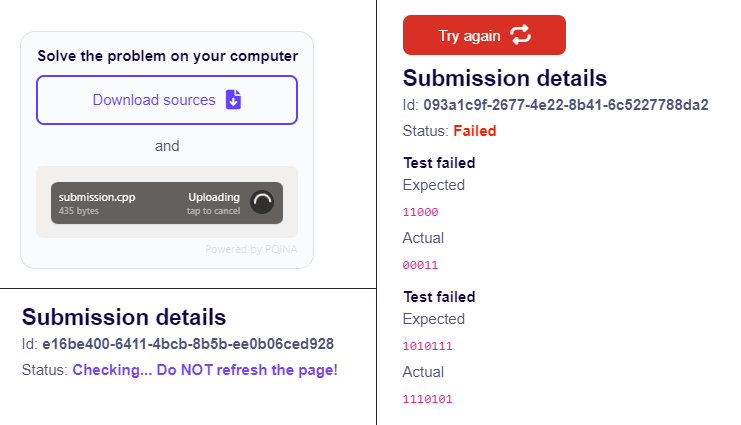
\includegraphics[width=300px]{./pics/submission-status.png}
	\caption{Submission status}
	\label{fig:submission-status}
\end{figure}

\section{Online workspaces}
The user can launch an online workspace directly from the problem solving page. The workspace is a Visual Studio Code instance that is running in the browser. The user can edit the source code of the solution and run it directly in the browser. The workspace is preconfigured with the necessary files and extensions for the problem.

\begin{figure}[h]
	\centering
	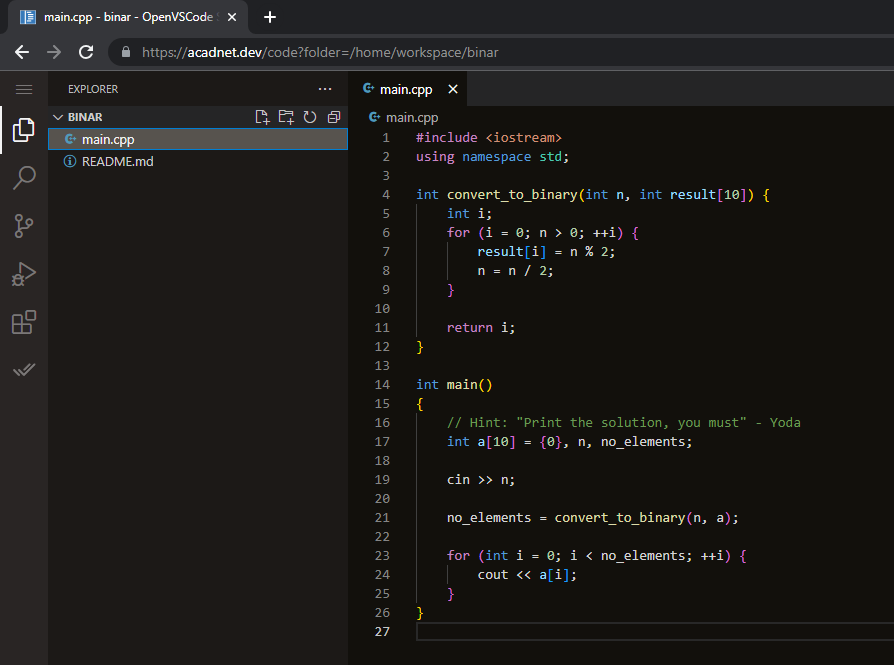
\includegraphics[width=\linewidth]{./pics/online-workspace.png}
	\caption{Online workspace}
	\label{fig:online-workspace}
\end{figure}


% DEPLOYMENT AND MAINTENANCE
\chapter{Deployment and maintenance}
\section{Infrastructure}
\subsection{Kubernetes cluster}
The entire platform was created with the idea of being scalable and responsive. The platform is deployed on a Kubernetes cluster managed by DigitalOcean. The cluster is composed of multiple Droplets\protect\footnotemark{}. DigitalOcean provides automatic horizontal scaling for the cluster, which means that the cluster can automatically add or remove nodes based on the load. The platform is configured to have a pool of a minimum of 2 Droplets at any time and a maximum of 5. The cluster is also configured to automatically restart the pods if they crash. This way, the platform is always available and responsive.
\footnotetext{A Droplet is a virtual machine on DigitalOcean}

A droplet has 2 vCPUs, 2GB RAM and 60GB SSD. The cluster is configured to automatically add new nodes if the CPU usage is above 70\% for more than 5 minutes. 

On the cluster, the following components are deployed.

\begin{itemize}
	\item \textbf{Web application} - the web application is deployed as a Docker image using multi-stage builds. The Docker image is deployed on the cluster using Helm Charts in an ArgoCD application.
	\item \textbf{Checker} - the checker is deployed as a Docker image. The Docker image is deployed on the cluster using Helm Charts in an ArgoCD application.
	\item \textbf{Workspaces manager} - the workspaces manager is deployed as a Docker image. The Docker image is deployed on the cluster using Helm Charts in an ArgoCD application.
	\item \textbf{Checker Sandboxes} - dynamic Pods that are created by the checker to evaluate the submissions. The Pods are created using the Kubernetes Python client.
	\item \textbf{VSCode Server} - dynamic Pods that are created by the workspaces manager to create the online workspaces. The Pods are created using the Kubernetes Python client.
\end{itemize}

\subsection{PostgreSQL}
The PostgreSQL database is deployed as a managed service on DigitalOcean Databases. The database is configured to automatically restart if it crashes and to automatically backup the data. The database is configured on a Digitalocean VPC (Virtual Private Cloud) so that it can be accessed only from the Kubernetes cluster. This way, the database is not exposed to the internet and it is more secure.

\subsection{File storage}
The storage used for the files is a managed service provided by DigitalOcean called Spaces. This S3 compatible storage organizes the files in buckets as objects. Like the database, the storage is configured on a Digitalocean VPC (Virtual Private Cloud) so that it can be accessed only from the Kubernetes cluster. This way, the storage is not exposed to the internet and it is more secure.


\section{Continuous integration}
All the components described in Chapter \ref{implementation-details} are built and tested using Github Actions. All the components, are built as Docker images and pushed to Github Container Registry. The Docker images are tagged with the commit hash and with the latest tag.

The building process is mostly the same for all the components. The only difference is the 'Dockerfile' used to build the image, because each component runs on its own environment. The building process is described below.

\begin{enumerate}
	\item Checkout the repository
	\item Login to Github Container Registry
	\item Replace variables in JSON configuration files with environment variables stored in Github Secrets
	\item Build the Docker image with layer caching
	\item Push the Docker image to Github Container Registry
\end{enumerate}

The Github Action is ran on every push to the main branch and on every pull request to the main branch.

\begin{figure}[h]
	\centering
	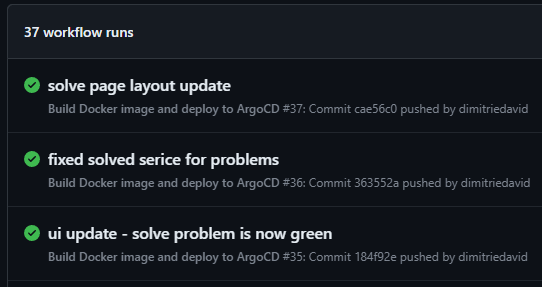
\includegraphics[width=200px]{./pics/github-actions-workflows.png}
	\caption{Example of Github Actions workflows running on multiple ocasions}
	\label{fig:github-actions-workflows}
\end{figure}

\section{ArgoCD}
ArgoCD is a tool that allows us to deploy Kubernetes manifests from a Git repository. It is used to deploy the Helm Charts for the web application, the checker, and the workspaces manager. The manifests are stored in the \href{https://github.com/acadnet-dev/infra}{acadnet-dev/infra} repository. The manifests are deployed automatically when a new commit is pushed to the repository, because ArgoCD is polling the repository for changes every 3 minutes.


\section{Continuous deployment}
All the components described in Chapter \ref{implementation-details} are deployed on the Kubernetes cluster using Helm Charts. The Helm Charts are deployed using ArgoCD. The deployment is done automatically at the end of the Github Actions build process. The deployment process is done by updating the image version in the ArgoCD deployment using the ArgoCD API.

\begin{figure}[h]
	\centering
	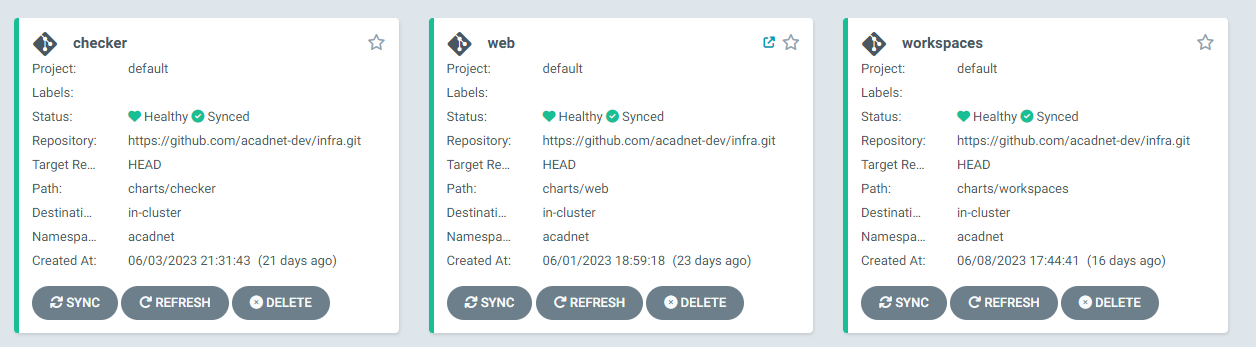
\includegraphics[width=400px]{./pics/argocd-apps.png}
	\caption{Applications deployed with ArgoCD}
	\label{fig:argocd-apps}
\end{figure}

\begin{figure}[h]
	\centering
	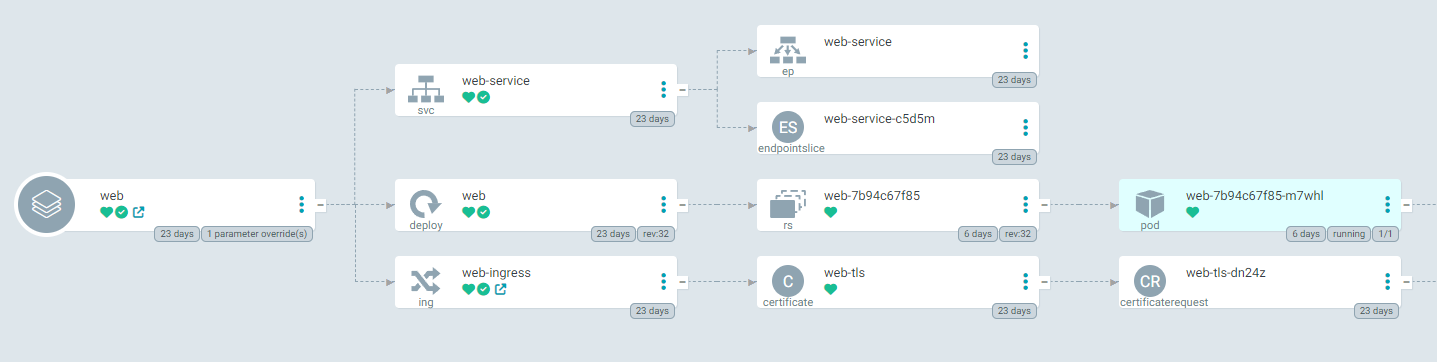
\includegraphics[width=400px]{./pics/argocd-web.png}
	\caption{Web application deployment}
	\label{fig:argocd-web}
\end{figure}

\newpage
\section{Monitoring}
Like any software application, monitoring is a very important aspect of the platform. Because of the complexity of the platform, it is difficult to monitor all applications individually. As just a little effort was put into monitoring, the platform is currently monitored only at a high level. When looking at the performance and resource usage, the monitoring is done using DigitalOcean's monitoring service. This service provides a dashboard with the CPU, memory and disk usage of the Droplets. The dashboard can be seen in Figure \ref{fig:monitoring-dashboard}. In terms of logging, the logs can be seen in a centralized place in ArgoCD. The logs are collected from the Kubernetes cluster and displayed in each application's dashboard like in Figure \ref{fig:argocd-logs}.

\begin{figure}[h]
	\centering
	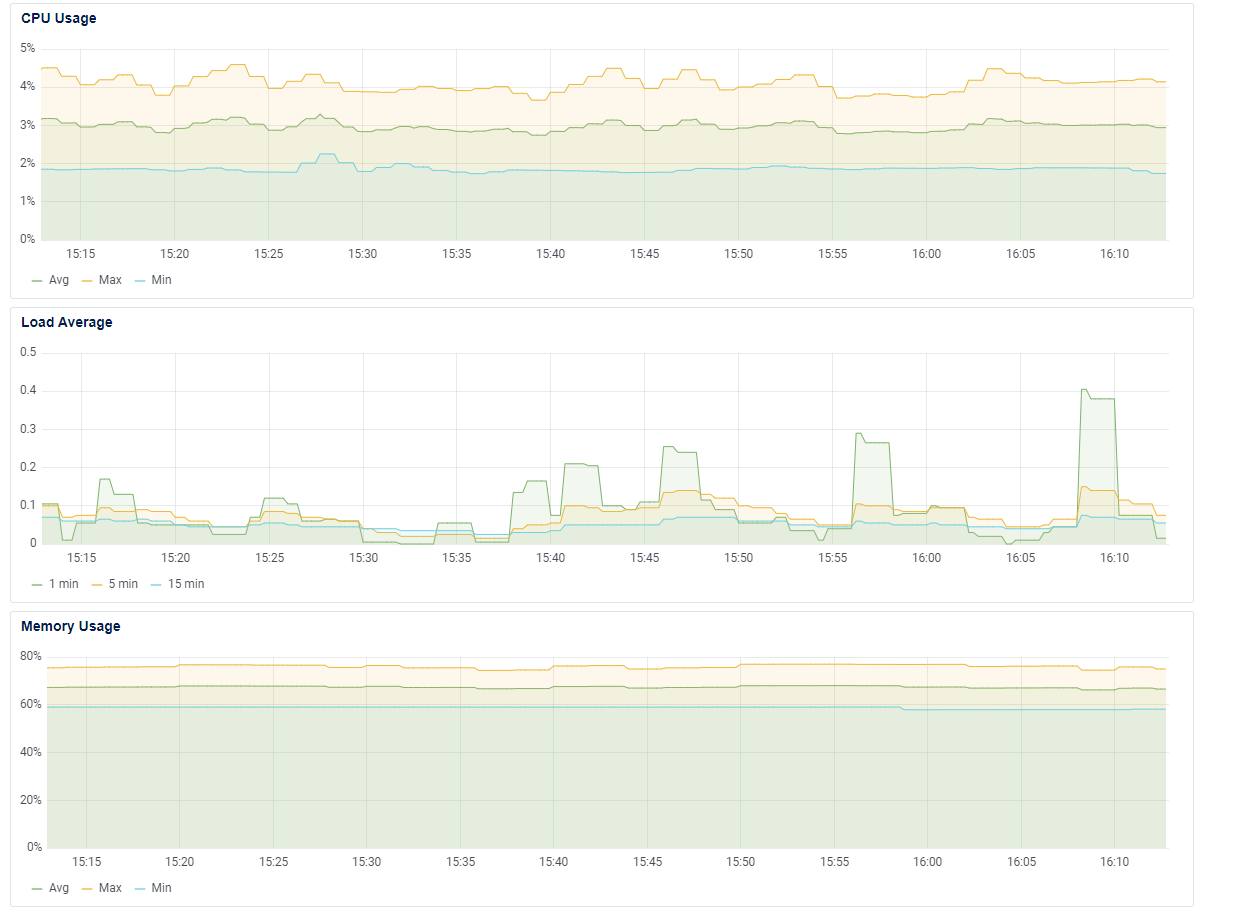
\includegraphics[width=400px]{./pics/monitoring-dashboard.png}
	\caption{Monitoring dashboard}
	\label{fig:monitoring-dashboard}
\end{figure}

\begin{figure}[h]
	\centering
	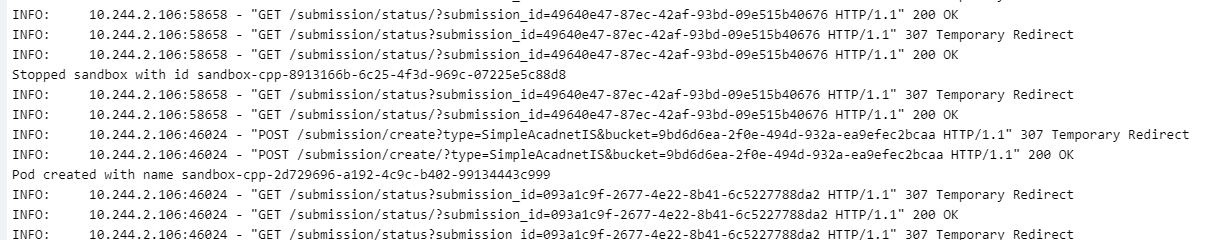
\includegraphics[width=400px]{./pics/argocd-logs.png}
	\caption{Logs for the checker}
	\label{fig:argocd-logs}
\end{figure}


% TESTING AND VALIDATION
\chapter{Testing and validation}
\section{Submission evaluation fairness}
An important aspect of submission evaluation is fairness. The platform needs to be fair to all the users. This means that the submission evaluation performance and results should be the same for all the users. This thing should be achieved under any load, for any hardware and for any number of users. This is a very difficult thing to achieve, because the platform is running on a Kubernetes cluster, which means that the pods are running on different nodes and the nodes have different hardware. The Kubernetes cluster is also configured to automatically scale the number of nodes based on the load, which means that the pods can be moved from one node to another at any time. This means that the pods can run on different hardware at any time.

To address this, the platform implements the following things.

\textbf{Same hardware for all the nodes}
All the nodes in the cluster are configured to have the same hardware. This means that all the pods will run on the same hardware, even if it is virutalized.

\textbf{Resource limits for sandbox deployments}
The sandbox deployments are configured to have resource limits and requests. This means that the pods will have the same amount of CPU and memory available, or the submission will not start and the cluster will need to scale up.

\textbf{Submissions ran separately}
The submissions are ran separately, which means that the pods will not interfere with each other. This means that the pods will not have to share the CPU and memory with other pods.

\textbf{Hand-crafted tests}
Authors are instructed to create tests that are not easily influenced by hardware resource fluctuations. For example, by limiting submission execution time and memory usage, we do not test the performance of the code, but the complexity of the algorithm. This way, the difference in performance between different complexities will be so big that it will not be influenced by the unpredictability of the hardware.

\section{Performance and scalability}
The platform is designed to be scalable and responsive. This means that the platform should be able to handle a large number of users and submissions. Being deployed on a Kubernetes cluster in a cloud environment, the platform can automatically scale up by spinning up new nodes. This comes with the downside of having unpredictable costs, because the number of nodes can change at any time.

The only problem is that spinning a new node takes a few minutes, which means that the user will have to wait a few minutes for the submission to start or for the workspace to open. Because of this, the platform is configured to have at least a free node (buffer node) at any time. This way, the user will not have to wait for the node to spin up. When this buffer node is used, the cluster will automatically spin up a new node to be available for the next scale up.

\section{Security}
\textbf{Networking}
The platform is deployed on a DigitalOcean VPC (Virtual Private Cloud). This means that the cluster is not exposed to the internet and it is more secure. The only thing that is exposed to the internet is the web application, which is exposed via a load balancer. The load balancer is configured to only allow traffic on port 80 and 443. The applications are talking between them using their internal IP addresses and ports.

\textbf{Certificates}
All the exposed endpoints are secured with SSL certificates. The certificates are automatically generated and renewed by Let's Encrypt, every 3 months.

\textbf{Authentication}
The users can authenticate using their Google account. This is done via the Google OAuth2 authentication provider. This way, the platform does not store any passwords and does not manage forgotten passwords.

\textbf{Authorization}
The platform has authorization based on user roles. The two roles are for authors and students. All the access is based on the user's journey. Each role's journey is described in Chapter \ref{user-journey}.

\section{Testing}
For testing purposes, the platform has already 6 problems uploaded. These problems are from the 2023 edition of the National Olympiad of Applied Informatics Acadnet. The problems statements are in Romanian and they are implemented using the only developed problem type, C++.

The platform was tested by multiple users. The users were asked to create an account and solve a problem, by uploading the solution and by solving directly in the online workspace. The users were asked to give feedback about the platform. The feedback was mostly positive. The users liked the platform and they found it easy to use. The users also found some bugs and suggested some improvements. The bugs were fixed and the improvements were added to the \ref{future-work} section.


% CONCLUSIONS AND FUTURE WORK
\chapter{Future work and conclusions}
\section{Future enhancements}
\label{future-work}
\textbf{More problem types}
\\
The platform can be extended to support more problem types. Currently, the only supported problem type is C++. The platform can be extended to support other languages like Java, Python, C\#, etc. As it is open-source and it is easy to extend, the platform can be extended by any author that wants to create problems for the platform.

\textbf{Automatical removal of workspaces}
\\
The workspaces are currently removed manually by the maintainer. The platform can be extended to automatically remove the workspaces after a period of inactivity. This way resources will be saved and the costs will be reduced.

\textbf{Persistent workspaces}
\\
The workspaces are currently not persistent. This means that the user will lose all the changes made to the workspace after the workspace is shut down. The platform can be extended to support persistent workspaces. This way, the user will be able to save the workspace and continue working on it later. Also, the available space in the workspace can be limited to a certain amount like 100MB. This way, the users will not be able to store large files in the workspace.

\textbf{Contests}
\\
The platform can be extended to support contests. This way, the platform can be used to organize contests for highschool students. The contests can be organized by the teachers and the students can participate in the contests. This includes a contest component that allows the teachers to create contests and to add existing problems to the contests. The contests can be open or private. The private contests can be accessed only by the students that are enrolled in the course. There should be a leaderboard and a monitoring component that allows the teachers to see the progress of the students during the contest.

\textbf{Private test results}
\\
Currently the test results are public. This means that the students can see the test results. The students may not be able to see the test results, because they can use hardcode the answer.

\textbf{Execution time and memory usage limits}
\\
At the moment, the submissions are not limited in terms of execution time and memory usage. This means that the submissions can run for as long as they want and they can use as much memory as they want. This can be a problem because the submissions can run for a long time and they can use a lot of memory. The platform can be extended to support execution time and memory usage limits. Also, this limit can be used by authors to create tests that check the complexity of the algorithm.

\textbf{C++ environment in workspaces}
\\
Currently, the workspaces are not configured to have a C++ environment. This means that the users cannot compile and run C++ directly in the virtual machine they are running inside. The workspace can have a C++ compiler and extensions for VS Code that allow the user to compile and run C++ directly in the workspace. This extension also provides syntax highlighting and code completion for C++. This can be extended for any implemented problem type.

\textbf{Management of authors}
\\
At the moment, the authors are assigned manually by the application administrator, by directly interacting with the database. An admin role can be added to the platform that allows the administrator to manage the authors. This includes adding new authors, removing authors and changing the author's role.

\textbf{Better UI/UX}
\\
The platform can be improved in terms of UI/UX. The current state of the UI is only a proof of concept. The UI can be improved to be more user friendly and allow more actions to be done directly from the UI.

\newpage
\section{Lessons learned}
Developing a complex project like this one requires a lot of planning. Unfortunately, I only created a bird's eye view of the project and I did not plan the implementation in detail. This led to a lot of time spent on research before actually starting the implementation of each component. Multiple functionality changes in the implementation were also caused because the planning was not done in detail. 

Another thing that I learned is that it is very important to have a clear vision of the project from the start. This way, less time is spent refactoring ideas and more time is spent writing quality code.

The last thing that I think had a big impact on writing this thesis is that during the implementation, I created multiple diagrams and I wrote a lot of documentation. This documentation can be found in the \href{https://github.com/acadnet-dev/docs}{acadnet-dev/docs} repository, together with the diagrams. This documentation helped me a lot when writing this thesis, because I did not have to remember why I made certain decisions. I just had to read the documentation and the diagrams and I remembered everything.

A really frustrating problem I encountered was debugging the Kubernetes pod manager that the checker and the workspace manager use to launch pods on the cluster, because it could be only tested in the production environment.

\section{Conclusions}
The platform is a success as it is easy to use and it is scalable. All the planned objectives were achieved. \href{https://acadnet.dev}{AcadNet.dev} will be hosted with the main purpose of being used by highschool students to learn programming and to prepare for the National Olympiad of Applied Informatics.

On the techincal side, there were multiple challanges, starting from selecting which technologies to use and ending with the deployment and maintenance of the platform. Interconnecting all the components was also a challange, because the platform is composed of multiple components written in different technologies.

Overall, I think that this project is a success. As it being the project for finishing univeristy, I think I used a lot of knowledge from many courses that I attended during my studies. I also learned a lot of new things from it, like how to plan a complex software architecture, new technologies, CI/CD, Kubernetes and last but not least, how to write a thesis where I can express my ideas and my work.


\chapter*{Appendices}\addcontentsline{toc}{chapter}{Appendices}
\begin{appendices}

\chapter{Code snippets}
\label{anexa:cod}
\section{Submission status JSON example}
\label{anexa:cod:json-submission}
\begin{lstlisting}[language=json,firstnumber=1]
{
	"submission_id": "330f946d-95d0-45da-bffd-a45996045ba1",
	"status": "finished",
	"build_status": "success",
	"test_results": [{
			"test_name": "test01.in",
			"passed": false,
			"status": "failed",
			"exec_result": {
				"actual": "00011",
				"ref": "11000"
			}
		}
	],
	"status_history": [{
			"status": "created",
			"timestamp": 1686422831.5370035
		},{
			"status": "creating sandbox",
			"timestamp": 1686422831.5370176
		},{
			"status": "pod created with name sandbox-cpp-5d8720e1-c042-43ea-a95a-e8e268c6f0be",
			"timestamp": 1686422831.570527
		},{
			"status": "waiting for sandbox to start - pod status: Pending",
			"timestamp": 1686422836.5834553
		},{
			"status": "sandbox launched",
			"timestamp": 1686422836.6700737
		},{
			"status": "uploading submission file",
			"timestamp": 1686422836.6700778
		},{
			"status": "compiling submission",
			"timestamp": 1686422836.685021
		},{
			"status": "uploading test test01.in",
			"timestamp": 1686422840.5165641
		},{
			"status": "running test test01.in",
			"timestamp": 1686422840.5247858
		},{
			"status": "comparing output for test test01.in",
			"timestamp": 1686422840.5364146
		},{
			"status": "finished",
			"timestamp": 1686422852.6135993
		}]
}
\end{lstlisting}


\end{appendices}
\end{document}